\section{Évolution de la performance des supercalculateurs}\label{sec:edl_evolution}
%%%%%%%%%%%%%%%%%%%%%%%%%%%%%%%%%%%%%%%%%%%%%%%%%%%%%%%%%%%

La performance des supercalculateurs a beaucoup évolué depuis leur apparition. Pour comprendre les défis que l'industrie doit relever pour poursuivre ces améliorations, nous nous sommes intéressés à l'évolution des performances des architectures ces 20 dernières années.


\subsection{Comparer la performance des supercalculateurs}
%%%%%%%%%%%%%%%%%%%%%%%%%%%%%%%%%%%%%%%%%%%%%

    Pour mesurer et comparer la performance des supercalculateurs, il est nécessaire d'avoir une application de référence. L'étalonnage (\textit{benchmarking}) est une pratique courante qui consiste à évaluer plusieurs solutions en leur faisant passer une épreuve commune. Dans le domaine informatique, cela permet de tester différentes architectures matérielles et d'évaluer leurs performances. Un des benchmarks les plus utilisés dans le domaine du HPC est celui développé par Jack Dongara en 1988: le benchmark HPL (High-Performance Linpack) \cite{Dongarra2003}. Ce benchmark est un code simple qui résout un système d'équations linéaires $Ax = B$, $A$ et $B$ étant deux matrices. Les performances évoluent linéairement avec le nombre de machines utilisées, car très peu de communications sont nécessaires. Le résultat est un nombre d'\gls{FLOPS} que la machine peut exécuter, ce qui rend la comparaison entre supercalculateurs aisée.
    Ce code permet de publier deux classements bisannuels: le Top500 et le Green500 (\autoref{fig:Top500}).

        \begin{figure}[b!]
                \centering
                \begin{subfigure}[t]{0.48\textwidth}
                    \centering
                    
\includegraphics[width=.4\linewidth]{images/Top500_logo.png}
                    \caption{\label{fig:Top500_logo}Top500}
                \end{subfigure}\hfill
            \begin{subfigure}[t]{0.48\textwidth}
                    \centering
                    
\includegraphics[width=.25\linewidth]{images/Green500_logo.png}
                    \caption{\label{fig:Green500_logo}Green500}
            \end{subfigure}
            \caption{\label{fig:Top500} Les classements du Top500 et du Green500 sont présentés deux fois par an lors de la conférence Supercomputing\protect\footnotemark}
        \end{figure}
        \footnotetext{\url{supercomputing.org/}}
        
    \subsubsection{Le Top500}\label{sec:Top500}
    %%%%%%%%%%%%%%%%%%%%%%%%%%%%%%%%%%%%%%%%%%%%%
        
        Le TOP500\footnote{\url{www.top500.org}} est un classement mondial qui classe, tous les 6 mois depuis 1993, les 500 supercalculateurs les plus puissants au monde. Ce classement se base sur le nombre maximum d'opérations flottantes qui peuvent être exécutées en une seconde (\gls{FLOPS}) lors de l'exécution du benchmark HPL. Cette unité a été choisie, car la grande majorité des codes utilisés dans les domaines précédemment cités exécutent des opérations sur des nombres flottants. Il s'avère donc judicieux de choisir ce dénominateur commun pour comparer les différentes architectures.

        Il faut cependant savoir que ce classement ne contient pas toutes les machines. En effet, certains industriels ne préfèrent pas apparaître dans ce classement. Stratégiquement parlant, il peut être intéressant de ne pas publier sa puissance de calcul et nous savons que certaines des infrastructures les plus puissantes n'y figurent pas. Cependant, ce classement permet d'apprécier les tendances que suivent la majorité des architectures.
        
        Au moment de l'écriture de ce manuscrit, le dernier classement disponible est celui de novembre 2019\footnote{Top500 novembre 2019 -  \url{www.top500.org/lists/2019/11/}}. Les principales caractéristiques des quatre premiers supercalculateurs sont présentées dans le \autoref{tab:top500}. Les États-Unis et la Chine possèdent chacun deux entrées et se partagent 70\% des performances totales du Top500 (32.3\% pour la Chine, 37.1\% pour les États-Unis). Concernant le système d'interconnexion, 6 des 10 premières entrées, ainsi que 141 des 500 supercalculateurs,  utilisent la technologie Infiniband.
        L'efficacité des supercalculateurs représente la capacité d'une plateforme à atteindre la performance théorique \verb|Rpeak|. Sur les 500 plateformes répertoriées, 100 d'entre elles ne parviennent pas à atteindre plus de 50\% de la performance théorique. Cette information est importante pour comprendre la difficulté qu'ont les applications à utiliser ces plateformes efficacement. Le benchmark \verb|HPL| est un code très simple, avec peu d'accès mémoire. Les applications réelles, plus complexes, ont beaucoup de mal à atteindre la performance théorique. Depuis quelques années, le classement du Top500 donne la performance d'un second benchmark (HPCG, voir \autoref{sec:hpcg}). Pour ce benchmark, plus fidèle aux comportements d'applications réelles, aucune des plateformes n'atteint une efficacité supérieure à 4\%. Pour avoir une meilleure vision de l'efficacité des plateformes, le classement du Green500 peut être consulté.


        \begin{table}
\centering
\resizebox{\textwidth}{!}{%
\begin{tabular}{|c|c|c|r|r|r|c|r|r|r|}
\hline
\rowcolor[HTML]{EFEFEF} 
\textbf{Pos.} & \textbf{Nom} & \multicolumn{1}{l|}{\cellcolor[HTML]{EFEFEF}\textbf{Country}} & \multicolumn{1}{l|}{\cellcolor[HTML]{EFEFEF}\textbf{Nb. coeurs}} & \multicolumn{1}{l|}{\cellcolor[HTML]{EFEFEF}\textbf{Coeurs accélérateur}} & \multicolumn{1}{l|}{\cellcolor[HTML]{EFEFEF}\textbf{Alimentation (MW)}} & \multicolumn{1}{l|}{\cellcolor[HTML]{EFEFEF}\textbf{Accélérateur}} & \multicolumn{1}{c|}{\cellcolor[HTML]{EFEFEF}\textbf{Rpeak}} & \multicolumn{1}{c|}{\cellcolor[HTML]{EFEFEF}\textbf{Rmax}} & \multicolumn{1}{c|}{\cellcolor[HTML]{EFEFEF}\textbf{Éfficacité}} \\ \hline
1 & Summit & United States & 2414592 & 2211840 & 10 & NVIDIA GPU & 200 & 148 & 0.74 \\ \hline
2 & Sierra & United States & 1572480 & 1382400 & 7 & NVIDIA GPU & 125 & 94 & 0.75 \\ \hline
3 & Sunway TaihuLight & China & 10649600 & 0 & 15 & None & 125 & 93 & 0.74 \\ \hline
4 & Tianhe-2A & China & 4981760 & 4554752 & 18 & Matrix-2000 & 100 & 61 & 0.61 \\ \hline
\end{tabular}%
}
\caption{Classement du Top500 de novembre 2019. Les puissances Rpeak (puissance théorique) et Rmax (puissance mesurée par HPL) sont données en pétaFLOPS ($10^{15}$ FLOPS). L'efficacité est le rapport entre Rmax et Rpeak.}
\label{tab:top500}
\end{table}
   
    \subsubsection{Le Green500}
    %%%%%%%%%%%%%%%%%%%%%%%%%%%%%
        
        Un second classement a vu le jour en 2007 appelé le Green500\footnote{Green500 - \url{www.top500.org/green500/}}. Il classe les supercalculateurs selon un critère d'efficacité énergétique. Cette efficacité mesure le nombre d'opérations sur un nombre flottant réalisé pour 1 watt d'énergie fourni au supercalculateur. 
    
        En effet, ces vingt dernières années, les évolutions technologiques et l'augmentation de la taille des supercalculateurs n'avaient pas de limite physique. Cette course à la performance n'était dictée que par les budgets disponibles pour leur construction. Ainsi, l'émergence de plateformes consommant de grandes quantités d'énergie et très peu efficaces a été constatée (voir le classement du Top500). 
        
        En novembre 2019\footnote{\url{www.top500.org/green500/lists/2019/11/}}, les 34 premiers supercalculateurs utilisent tous des accélérateurs. La majorité étant des GPU Nvidia Tesla. Il est intéressant de noter que la deuxième place du classement est tenue par une plateforme basée sur le processeur PEZY-SC2 conçu par l'entreprise PEZY et fabriqué par TSMC. Seul le premier du classement n'utilise pas d'accélérateurs (voir \autoref{tab:green500}). Il utilise un processeur ARM basse fréquence pouvant exécuter des instructions vectorielles SVE (Scalable Vector Extensions) sur 512 bits.

        
        \begin{table}
            \centering
            \resizebox{0.80\textwidth}{!}{%
            \begin{tabular}{|c|r|l|l|r|r|r|r|}
            \hline
            \rowcolor[HTML]{EFEFEF} 
            \textbf{Position} & \multicolumn{1}{c|}{\cellcolor[HTML]{EFEFEF}\textbf{TOP500}} & \multicolumn{1}{c|}{\cellcolor[HTML]{EFEFEF}\textbf{Processeur}} & \multicolumn{1}{c|}{\cellcolor[HTML]{EFEFEF}\textbf{Accélérateur}} & \multicolumn{1}{c|}{\cellcolor[HTML]{EFEFEF}\textbf{Rmax}} & \multicolumn{1}{c|}{\cellcolor[HTML]{EFEFEF}\textbf{Rpeak}} & \multicolumn{1}{c|}{\cellcolor[HTML]{EFEFEF}\textbf{Efficacité}} & \multicolumn{1}{c|}{\cellcolor[HTML]{EFEFEF}\textbf{Efficacité énergétique}} \\ \hline
            1 & 159 & Fujitsu A64FX & Aucun & 1.99 & 2.35 & 0.84 & 16.876 \\ \hline
            2 & 420 & Xeon D-1571 & PEZY-SC2 700Mhz & 1.30 & 1.79 & 0.72 & 16.256 \\ \hline
            3 & 24 & IBM POWER9 & Volta GV100 & 8.04 & 11.12 & 0.72 & 15.771 \\ \hline
            4 & 373 & IBM POWER9 & Tesla V100 SXM2 & 1.46 & 1.73 & 0.84 & 15.574 \\ \hline
            \end{tabular}%
            }
            \caption{Classement du Green500 de novembre 2019 selon l'efficacité énergétique (en gigaFLOPS/Watts). Les puissances Rpeak (puissance théorique) et Rmax (puissance mesurée par HPL) sont données en pétaFLOPS ($10^{15}$ FLOPS).}
            \label{tab:green500}
        \end{table}
        
        
\subsection{Évolution des performances des supercalculateurs}
%%%%%%%%%%%%%%%%%%%%%%%%%%%%%%%%%%%%%%

    Le classement du Top500 a de nombreux avantages, dont celui de promouvoir le HPC au grand public. Cependant, un effet de bord de ce classement est de motiver les constructeurs pour développer des architectures ayant de bonnes performances lors de l'exécution du benchmark HPL. Or, ce code n'est pas représentatif des applications réelles et nous pouvons nous demander si son utilisation pour l'établissement du Top500 n'a pas été contre-productive. Bien que certains des supercalculateurs les plus puissants n'y figurent pas, l'évolution du Top500 permet d'obtenir un aperçu des évolutions de performances des architectures.
    
    Pour avoir une vision globale de son évolution, nous étudions la performance cumulée des 500 supercalculateurs depuis le premier classement (voir \autoref{pic_top500perf_evo}). Nous distinguons deux phases: avant et après 2012. 
    Les performances du Top500 ont évolué d'un facteur 1000 tous les 11 ans, conformément aux performances prédites par la loi de Moore. À partir de 2013, il faut attendre en moyenne 20 ans pour voir la performance des supercalculateurs augmenter dans la même proportion.
    Dans cette section, nous discutons des différents facteurs qui ont permis l'évolution constante des performances des architectures pendant près de 20 ans et étudions les freins qui empêchent de poursuivre ce rythme. La majorité des améliorations évoquées sont présentées dans l'\aref{chap:sota:materiel}.

    
    \begin{figure}
        \center
        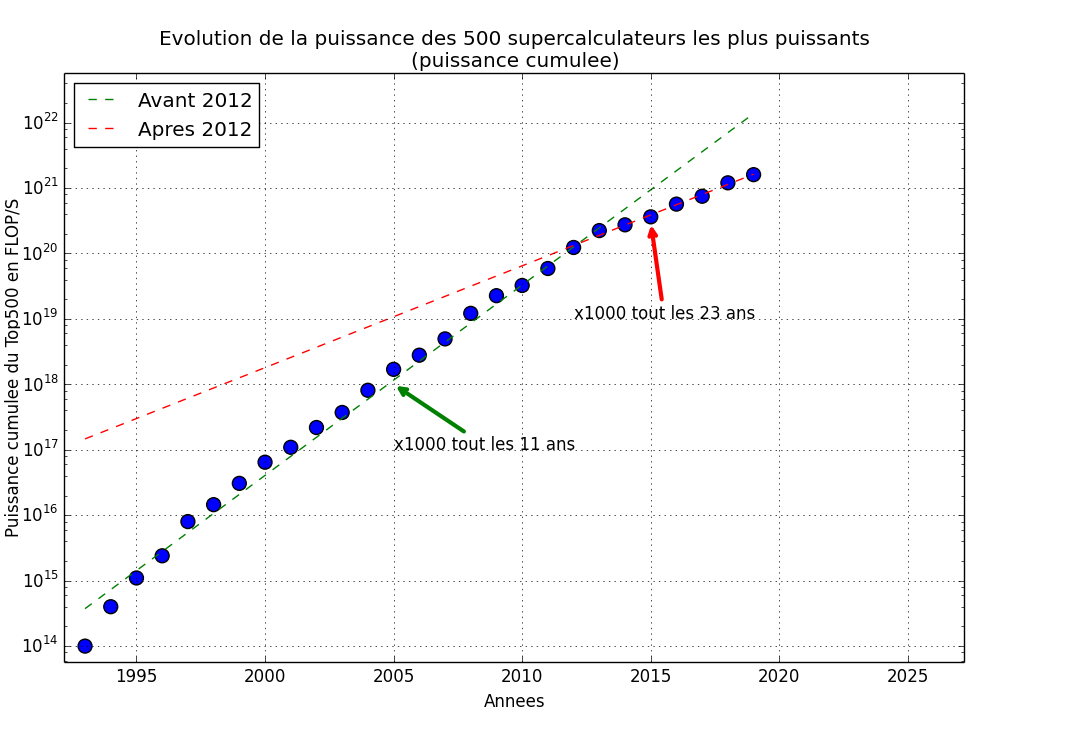
\includegraphics[width=12cm]{images/top500_evolution.png}
        \caption{\label{pic_top500perf_evo} Évolution de la performance cumulée des 500 supercalculateurs les plus puissants au monde. La pente de l'évolution diminue à partir de 2012.}
    \end{figure}


    \subsubsection{Avant 2012}\label{sec:proc_evo_2012}
    %%%%%%%%%%%%%%%%%%%%%%%%%%%%
    
        Les supercalculateurs ont pu bénéficier de nouvelles technologiques ainsi que de nombreuses innovations techniques.
        
        \begin{figure}[t!]
            \centering
            \begin{subfigure}[t]{0.33\textwidth}
                \centering
                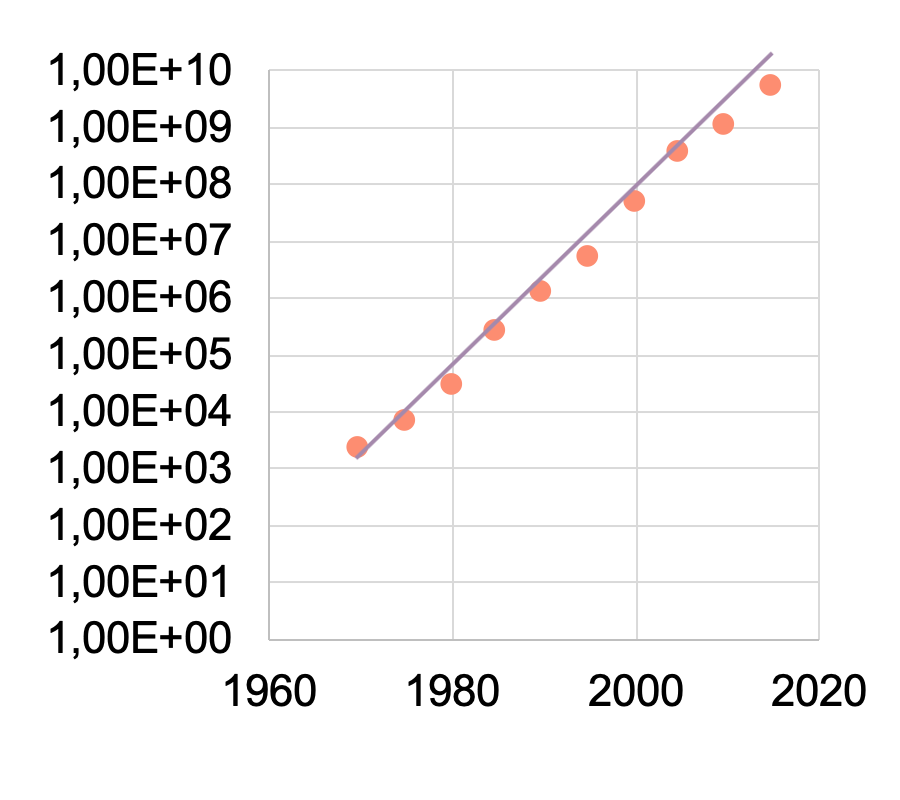
\includegraphics[width=\linewidth]{images/evo_transistor.png}
                \caption{\label{fig:evo_transistor}Évolution du nombre de transistors (\autoref{sec:denard})}
            \end{subfigure}\hfill
            \begin{subfigure}[t]{0.33\textwidth}
                \centering
                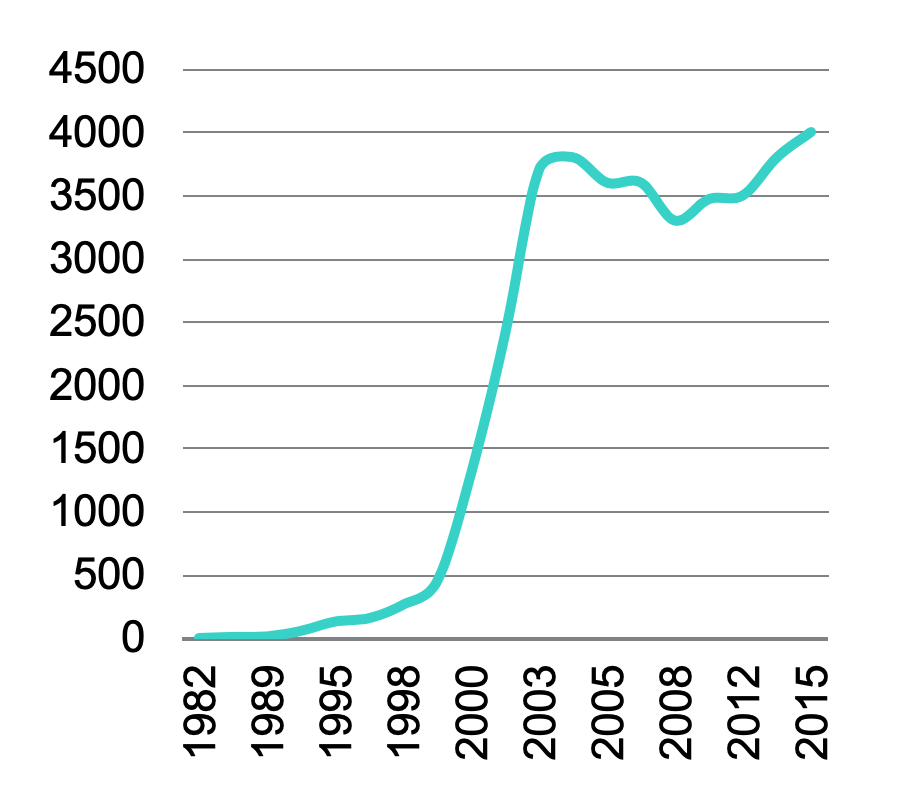
\includegraphics[width=\linewidth]{images/evo_freq.png}
                \caption{\label{fig:evo_freq}Évolution de la fréquence (\autoref{sec:frequency})}
            \end{subfigure}\hfill
            \begin{subfigure}[t]{0.33\textwidth}
                    \centering
                    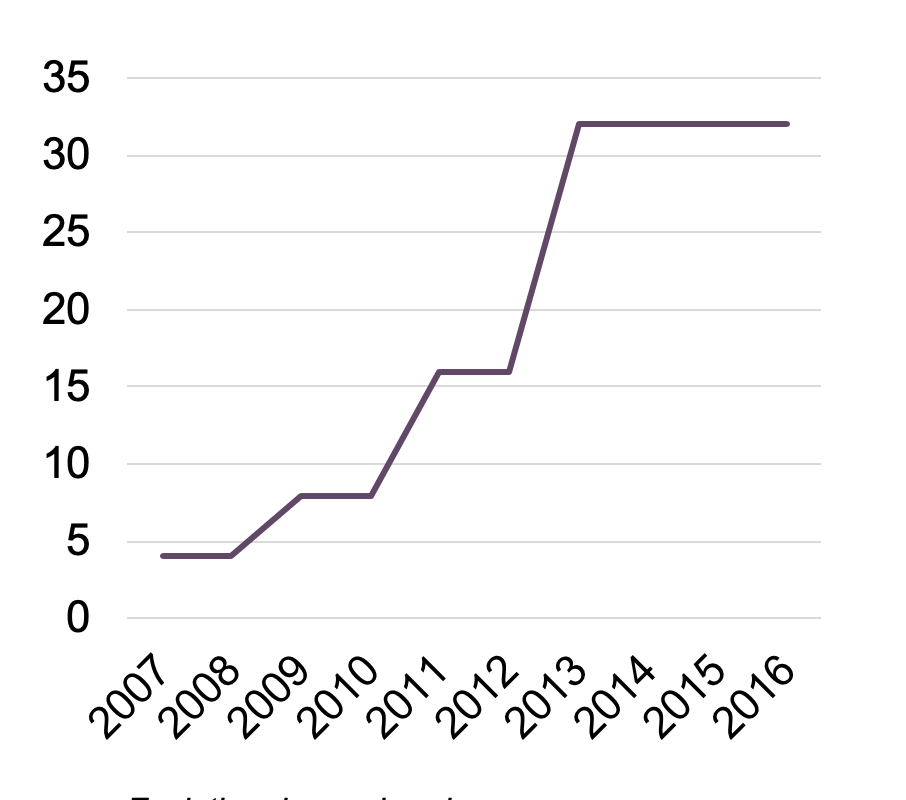
\includegraphics[width=\linewidth]{images/evo_core.png}
                    \caption{\label{fig:evo_core}Évolution du nombre de coeurs (\autoref{sec:multicore})}
            \end{subfigure}
            \caption{\label{fig:evo_proc}Évolutions technologiques principales des processeurs. Ces différentes évolutions sont présentées dans l'\aref{annexe:CHAPITRE_ARCHITECTURE}.}
        \end{figure}
        
            \paragraph{Les processeurs.} Dans l'\aref{chap:sota:materiel}, nous présentons les différentes évolutions technologiques dont ont pu bénéficier les processeurs. La \autoref{fig:evo_proc} résume les trois principales évolutions.
            Grâce à l'affinement des procédés de gravure, le nombre de transistors a évolué exponentiellement (voir \autoref{fig:evo_transistor}).  
            En miniaturisant les transistors et en utilisant des systèmes de refroidissement plus efficaces, la fréquence des processeurs a pu être augmentée de plusieurs facteurs (voir \autoref{fig:evo_freq}).
            Lorsque la fréquence n'a plus pu être augmentée, les architectures parallèles ont été développées, donnant naissance aux processeurs multicoeurs (voir \autoref{fig:evo_core}). La microarchitecture elle-même a reçu de nombreuses améliorations: l'utilisation de pipeline (voir \aref{sec:pipeline}) pouvant être superscalaire (voir \aref{sec:superscalar}), ainsi que le développement d'unités de calculs pouvant exécuter des instructions vectorielles (voir \aref{sec:cpu_vectoriel}).
            
            \paragraph{Les mémoires.} La performance des processeurs évoluant, celle des mémoires a aussi dû être améliorée pour fournir les données nécessaires aux traitements plus rapidement. Les principales améliorations sont dues à l'utilisation de nouvelles technologies mémoire (voir \autoref{sec:memory}), l'augmentation du nombre de canaux reliant la mémoire au processeur ou encore l'implémentation d'une hiérarchie de mémoire (voir \autoref{sec:hierarchie_true}). Celle-ci permettant aux applications de profiter du principe de localité (voir \autoref{sec:locality}).
            
        
    \subsubsection{Après 2012}
    %%%%%%%%%%%%%%%%%%%%%%%%%%%%
    
        En étudiant l'évolution de la puissance des supercalculateurs (voir \autoref{pic_top500perf_evo}), nous remarquons un ralentissement à partir des années 2010-2012. Ce ralentissement n'est pas dû à un seul facteur, mais à un ensemble de contraintes. En effet, les leviers et évolutions technologiques qui permettaient de tenir cette cadence ne sont plus disponibles aujourd'hui ou sont en fin de course (voir \autoref{fig:evo_proc}). Si certaines lois ont assuré une évolution continue de la performance des processeurs pendant plusieurs dizaines d'années, une partie du ralentissement de l'évolution des performances du Top500 peut être expliquée par leur \textit{essoufflement} \cite{FrancoisBodin2015}.

       
        \begin{figure}
            \center
            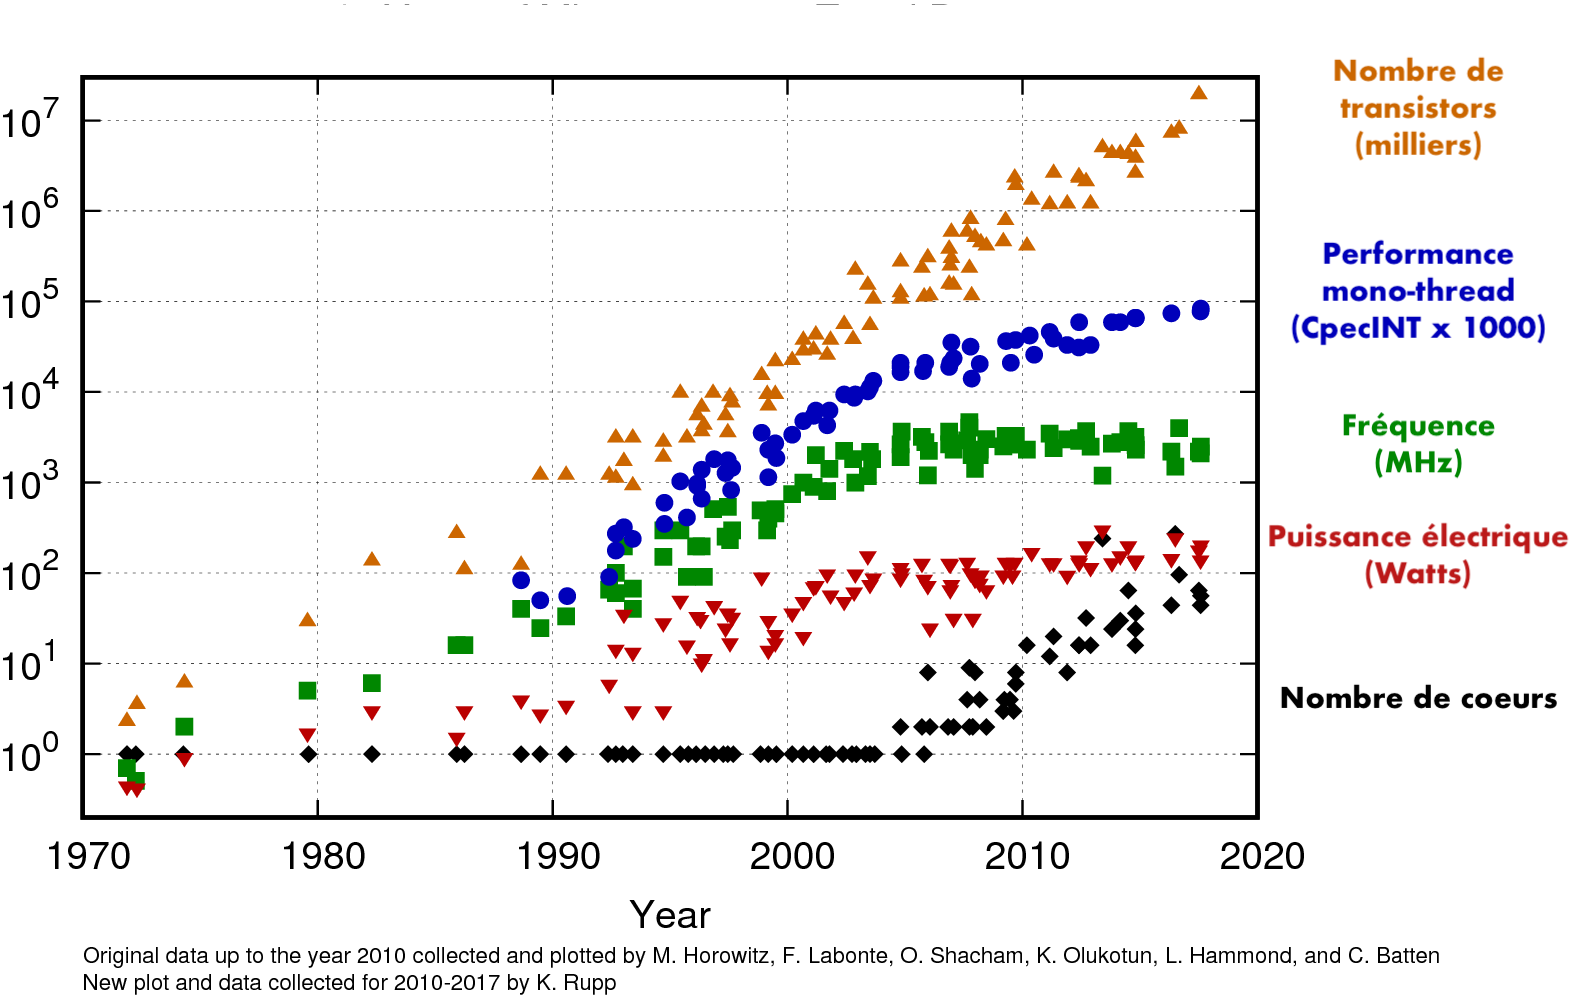
\includegraphics[width=12cm]{images/evo_proc.png}
            \caption{\label{fig:evo_cpu} Évolution des principales caractéristiques des processeurs (données originales tirées de \cite{rupp40years}\protect\footnotemark).}
        \end{figure}
        \footnotetext{Les données sont accessibles sur le dépôt GitHub de l'auteur:  \url{https://github.com/karlrupp/microprocessor-trend-data}}
        
%%%%%%%%%%%%%%%%%%%%%%%%%%%%%%%%%%%%%%%%%%%%%%%%%%%%%%%%%%%%%%%%%%%%%%%%%%%% 
      
        \paragraph{Fin de validité de la loi de Moore.}\label{sec:end_mooore} 
            
            La loi de Moore \cite{Moore1998} prévoyait que les architectures pourraient doubler leur nombre de transistors, tous les deux ans \cite{Moore75}, à coût constant (voir \autoref{sec:moore}). Malheureusement, les fondeurs ne parviennent plus à suivre le rythme dicté par la loi énoncée par Gordon Moore, pour des raisons principalement techniques (gravure), de coût \cite{Brooks2017} et de limite physique. La miniaturisation continue des transistors, dont la taille actuelle est de quelques nanomètres, rend la circulation des courants électriques instable. La bonne circulation des signaux électriques dans les circuits ne pouvant plus être garantie, il n'est alors plus possible de réduire leur taille.
            À partir de 2013, l'évolution des performances du Top500 passe pour la première fois sous les performances prévues par la loi de Moore (\autoref{fig:moore_vs_top500}).
            

            \begin{figure}
            \center
            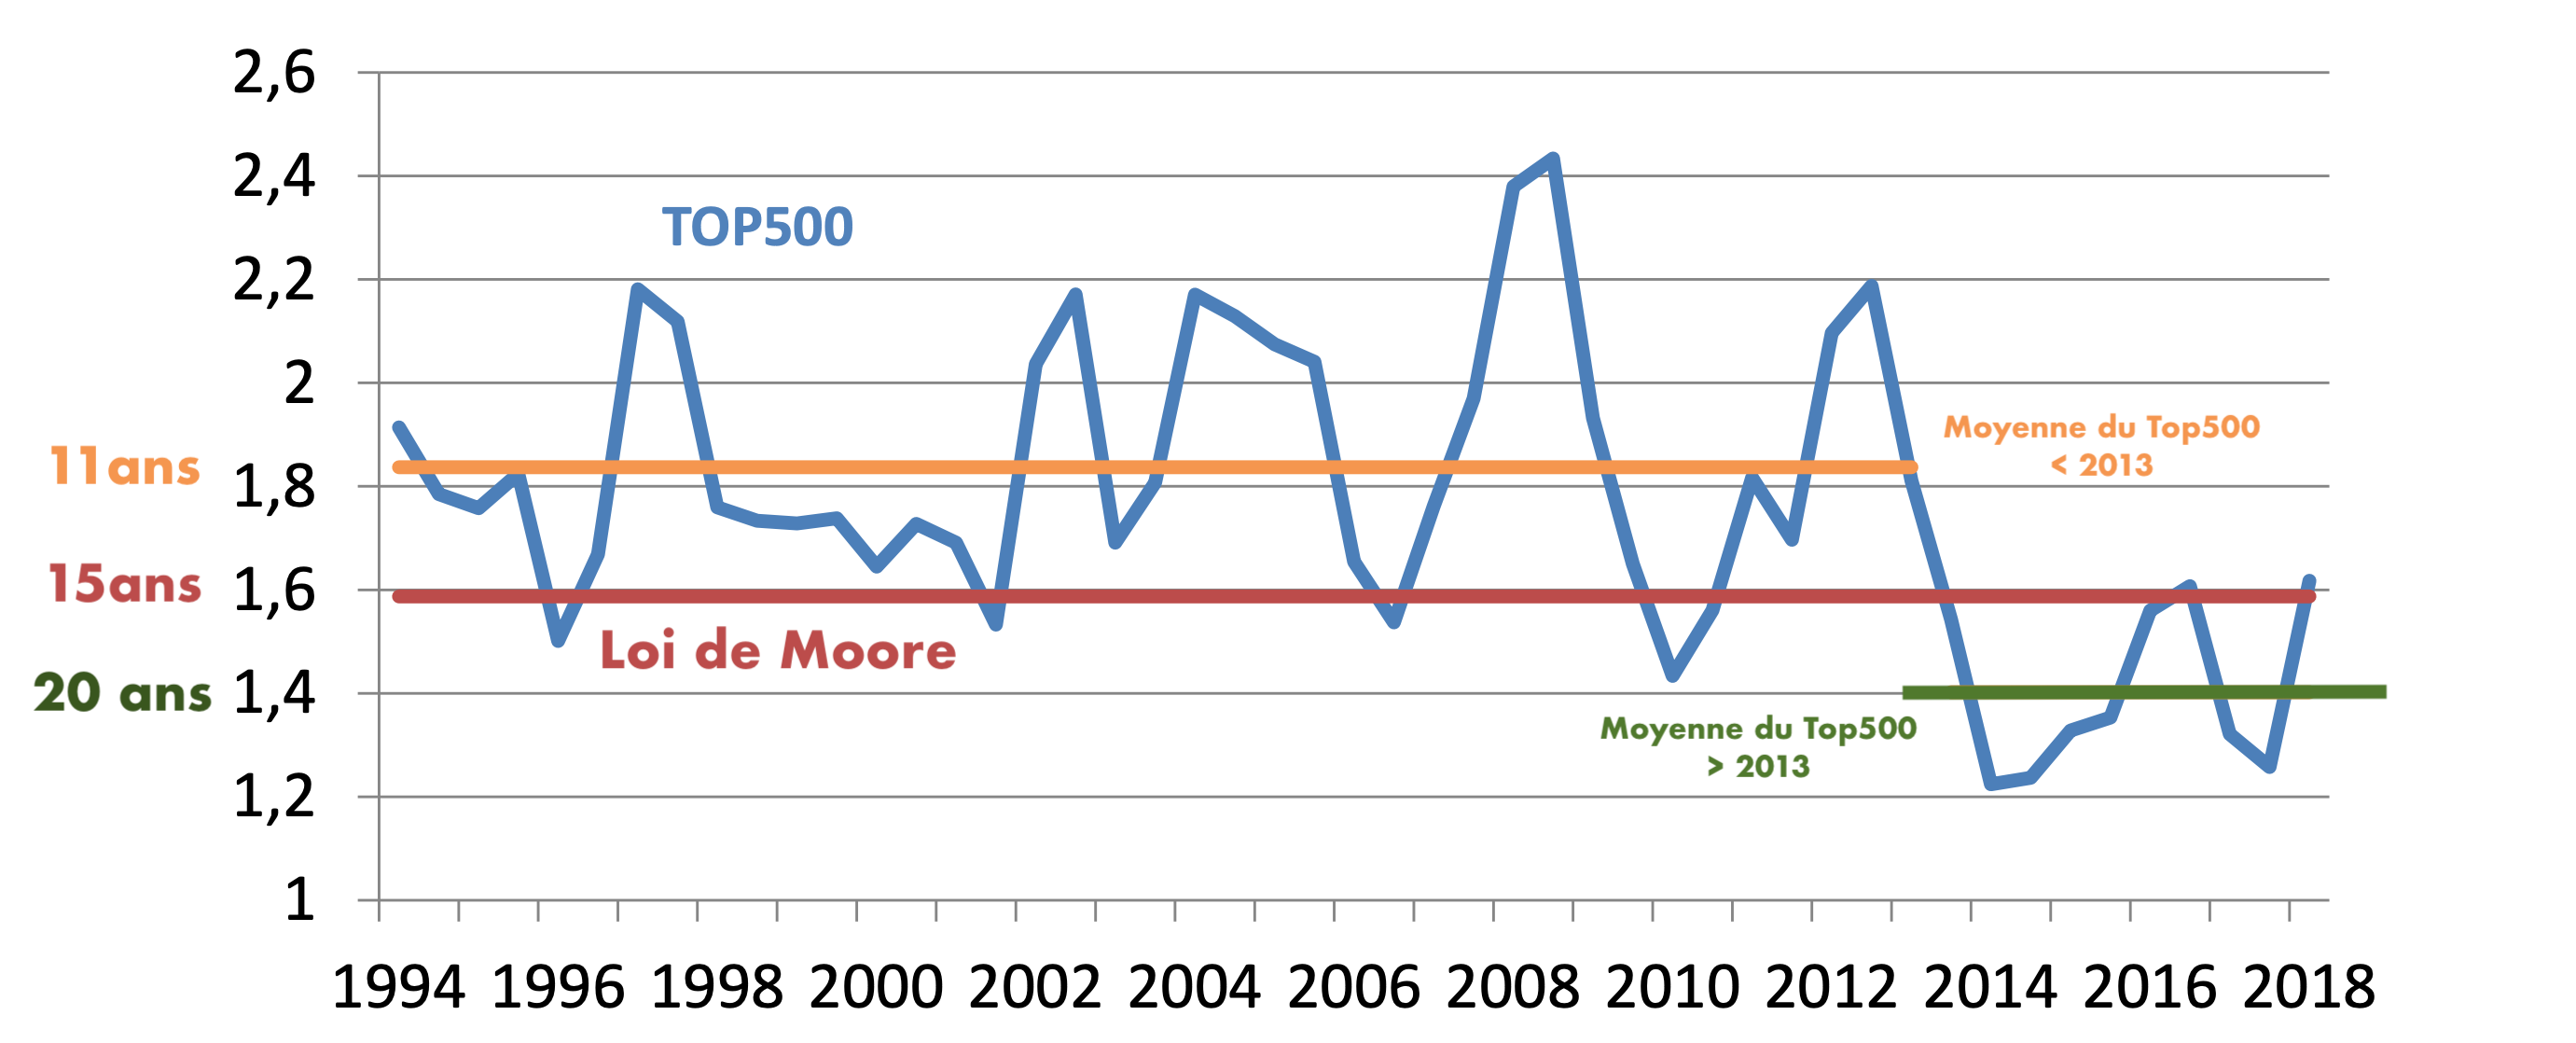
\includegraphics[width=16cm]{images/moore_vs_top500.png}
            \caption{\label{fig:moore_vs_top500}
             Facteur d'évolution annuelle des performances du Top500\protect\footnotemark. Jusqu'à 2013 la performance moyenne du Top500 évoluait d'un facteur 1.8, supérieur à l'évolution prédite par la loi de Moore (facteur 1.6). }
                \end{figure}
            \footnotetext{Graphique inspiré de la présentation du Top500 lors de la conférence ISC18 - \textit{Highlights of the 51st TOP500 List}}

        \paragraph{Fin de la validé de la loi de Dennard.} 
                
            Dans l'\aref{sec:denard}, nous avons discuté de l'augmentation de la fréquence des processeurs et introduit \textbf{la loi de Dennard} \cite{Dennard1974}. Ces équations ont prédit l'augmentation de la fréquence des processeurs de 40\% tous les 2 ans pendant plus de 30 ans. À cause des courants de fuite \cite{Wulf1995} augmentant exponentiellement avec la finesse de gravure des transistors, la consommation électrique des processeurs a elle aussi augmenté. Dans la \autoref{sec:denard}, nous expliquons comment la réduction de la taille des transistors et l'augmentation de la fréquence des processeurs augmentent la consommation électrique de circuit. L'énergie utilisée par le processeur étant dissipée sous forme de chaleur, il est devenu très difficile de refroidir ces architectures. De plus, l'énergie nécessaire pour le refroidissement a un impact sur la consommation. Cette limitation physique empêchant d'augmenter la puissance électrique des processeurs est appelée \textit{power wall} \cite{Kuroda2001}.

        \paragraph{Budget.} 
            
            Le prix des supercalculateurs est un frein à la construction de centres toujours plus puissants. Les calculateurs les moins puissants du classement sont généralement ceux dont le budget est le plus faible. Grâce à l'analyse du Top500, nous pouvons estimer que l'économie est un des freins participant au ralentissement de l'évolution des performances des architectures (voir \autoref{fig:Top500_Poor}). Le décrochage des performances du Top500, autour de 2012, étudié dans la section précédente intervient plus de 4 ans après le décrochage du dernier du classement (en 2008). De plus, on peut étudier la répartition de la performance du Top500 entre les supercalculateurs. En 2004, il fallait agréger les 80 premiers supercalculateurs du classement pour obtenir la moitié de la performance cumulée du Top500. En 2019, il faut seulement cumuler la puissance des 28 premiers. Ceci montre que les plateformes en haut du classement ont tendance à augmenter leur performance plus vite que celles du bas.
            
            
    
            \begin{figure}
            \center
            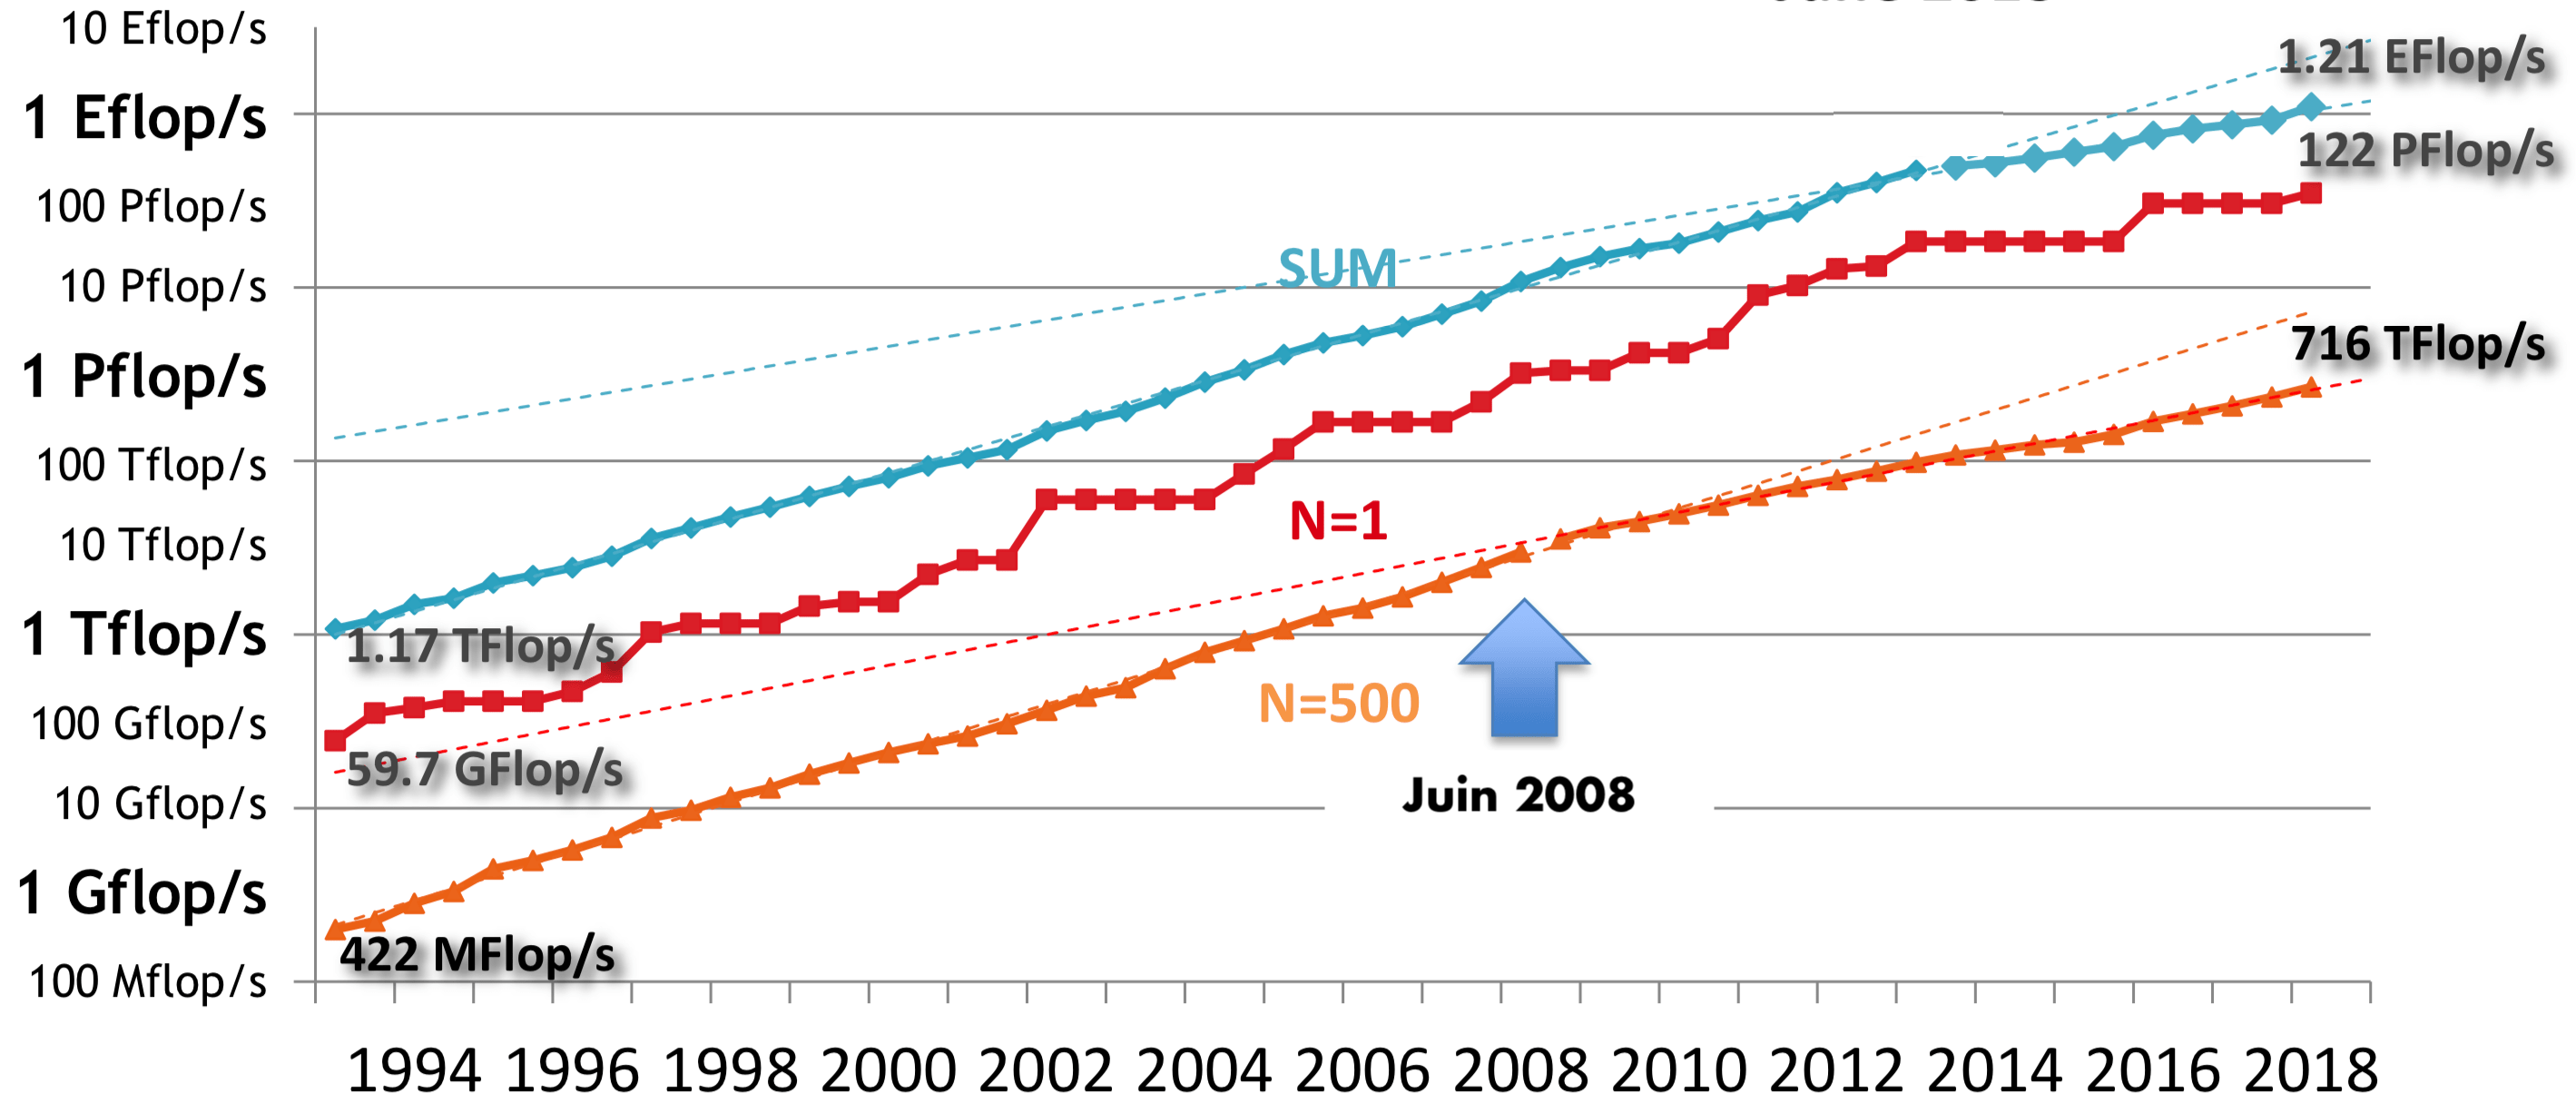
\includegraphics[width=14cm]{images/Top500_Poor.png}
            \caption{\label{fig:Top500_Poor} Évolution des performances du Top500 en \gls{FLOPS} grâce à l'aide du benchmark HPL. Le graphe présente la puissance cumulée des 500 ordinateurs (en bleu), celle du premier (en rouge) et celle du dernier (en orange)\protect\footnotemark.}
            \end{figure}
            \footnotetext{Graphique tiré de \url{https://www.top500.org/news/112019-highlights/}}
    
                
%%%%%%%%%%%%%%%%%%%%%%%%%%%%%%%%%%%%%%%%%%%%%%%%%%%%%%%%%%%%%%%%%%%%%%%%%%%% 
            
        \paragraph{Déséquilibre des microarchitectures.}  \label{sec:desequilibre_archi}
        Si l'utilisation de processeurs multicoeurs a permis de continuer d'augmenter la performance des processeurs malgré la faible évolution des fréquences, l'ajout de coeur a lui aussi atteint ses limites. En effet, comme démontré dans la \autoref{sec:parallele_perf}, l'augmentation des niveaux de parallélisme atteint elle aussi ses limites lorsque les applications contiennent des zones de codes séquentiels. Même des applications comme le benchmark \verb|HPL| sont impactés par \textbf{la loi d'Amdahl}, et l'ajout de coeurs s'est révélé de moins en moins efficace. On remarque sur la \autoref{fig:evo_cpu} que le nombre de coeurs a peu évolué ces dix dernières années. Dans l'\aref{sec:memory_wall_gap}, nous discutons de la disparité des évolutions technologiques des processeurs d'une part et des mémoires d'autre part. Cet écart a évolué au fil des années et il est aujourd'hui appelé \textit{mur de la mémoire} \cite{Rojas1997}  (\textit{memory wall} ou \textit{memory gap}). Les premiers processeurs étaient limités par la puissance de calcul, aujourd'hui il est très rare que la performance des applications de calcul haute performance soit limitée par celle des \gls{FPU}. L'ajout supplémentaire de coeurs est donc moins bénéfique, car le ratio de bande passante disponible par coeur diminue. 
        En étudiant l'évolution des performances des différentes parties du système, nous observons alors de réelles différences:             
        \begin{itemize}                 
            \item La performance calculatoire des processeurs (le nombre d'opérations flottantes réalisables par cycle) a \textbf{augmenté de 50\%} en moyenne par an.
            \item La bande passante entre le processeur et la mémoire a augmenté de 23\% par an                 
            \item La latence des requêtes mémoires a \textbf{diminué de 4\% } par an                 
            \item La bande passante sur le réseau a \textbf{augmenté de 20\%} par an             
        \end{itemize}
            
            La \autoref{pic:cpuvsmemory2} montre le déséquilibre entre ces deux parties fondamentales des architectures Von Neumann. Ce déséquilibre empêche aujourd'hui le système mémoire de transférer les données suffisamment rapidement pour que la totalité des unités de calculs soit constamment active. Pourtant, 50\% des broches d'un processeur récent sont allouées au système mémoire. Ainsi, bien que les performances de calculs des processeurs s'améliorent, les applications ne peuvent pas en bénéficier. La plupart des supercalculateurs atteignent rarement une efficacité de 80\% sur une application simple comme Linpack \cite{Dongarra2003}. Pour des applications réelles, cette efficacité est encore plus faible, parfois inférieure à 10\% \cite{Oliker2005}.
            
            \begin{figure}             \center             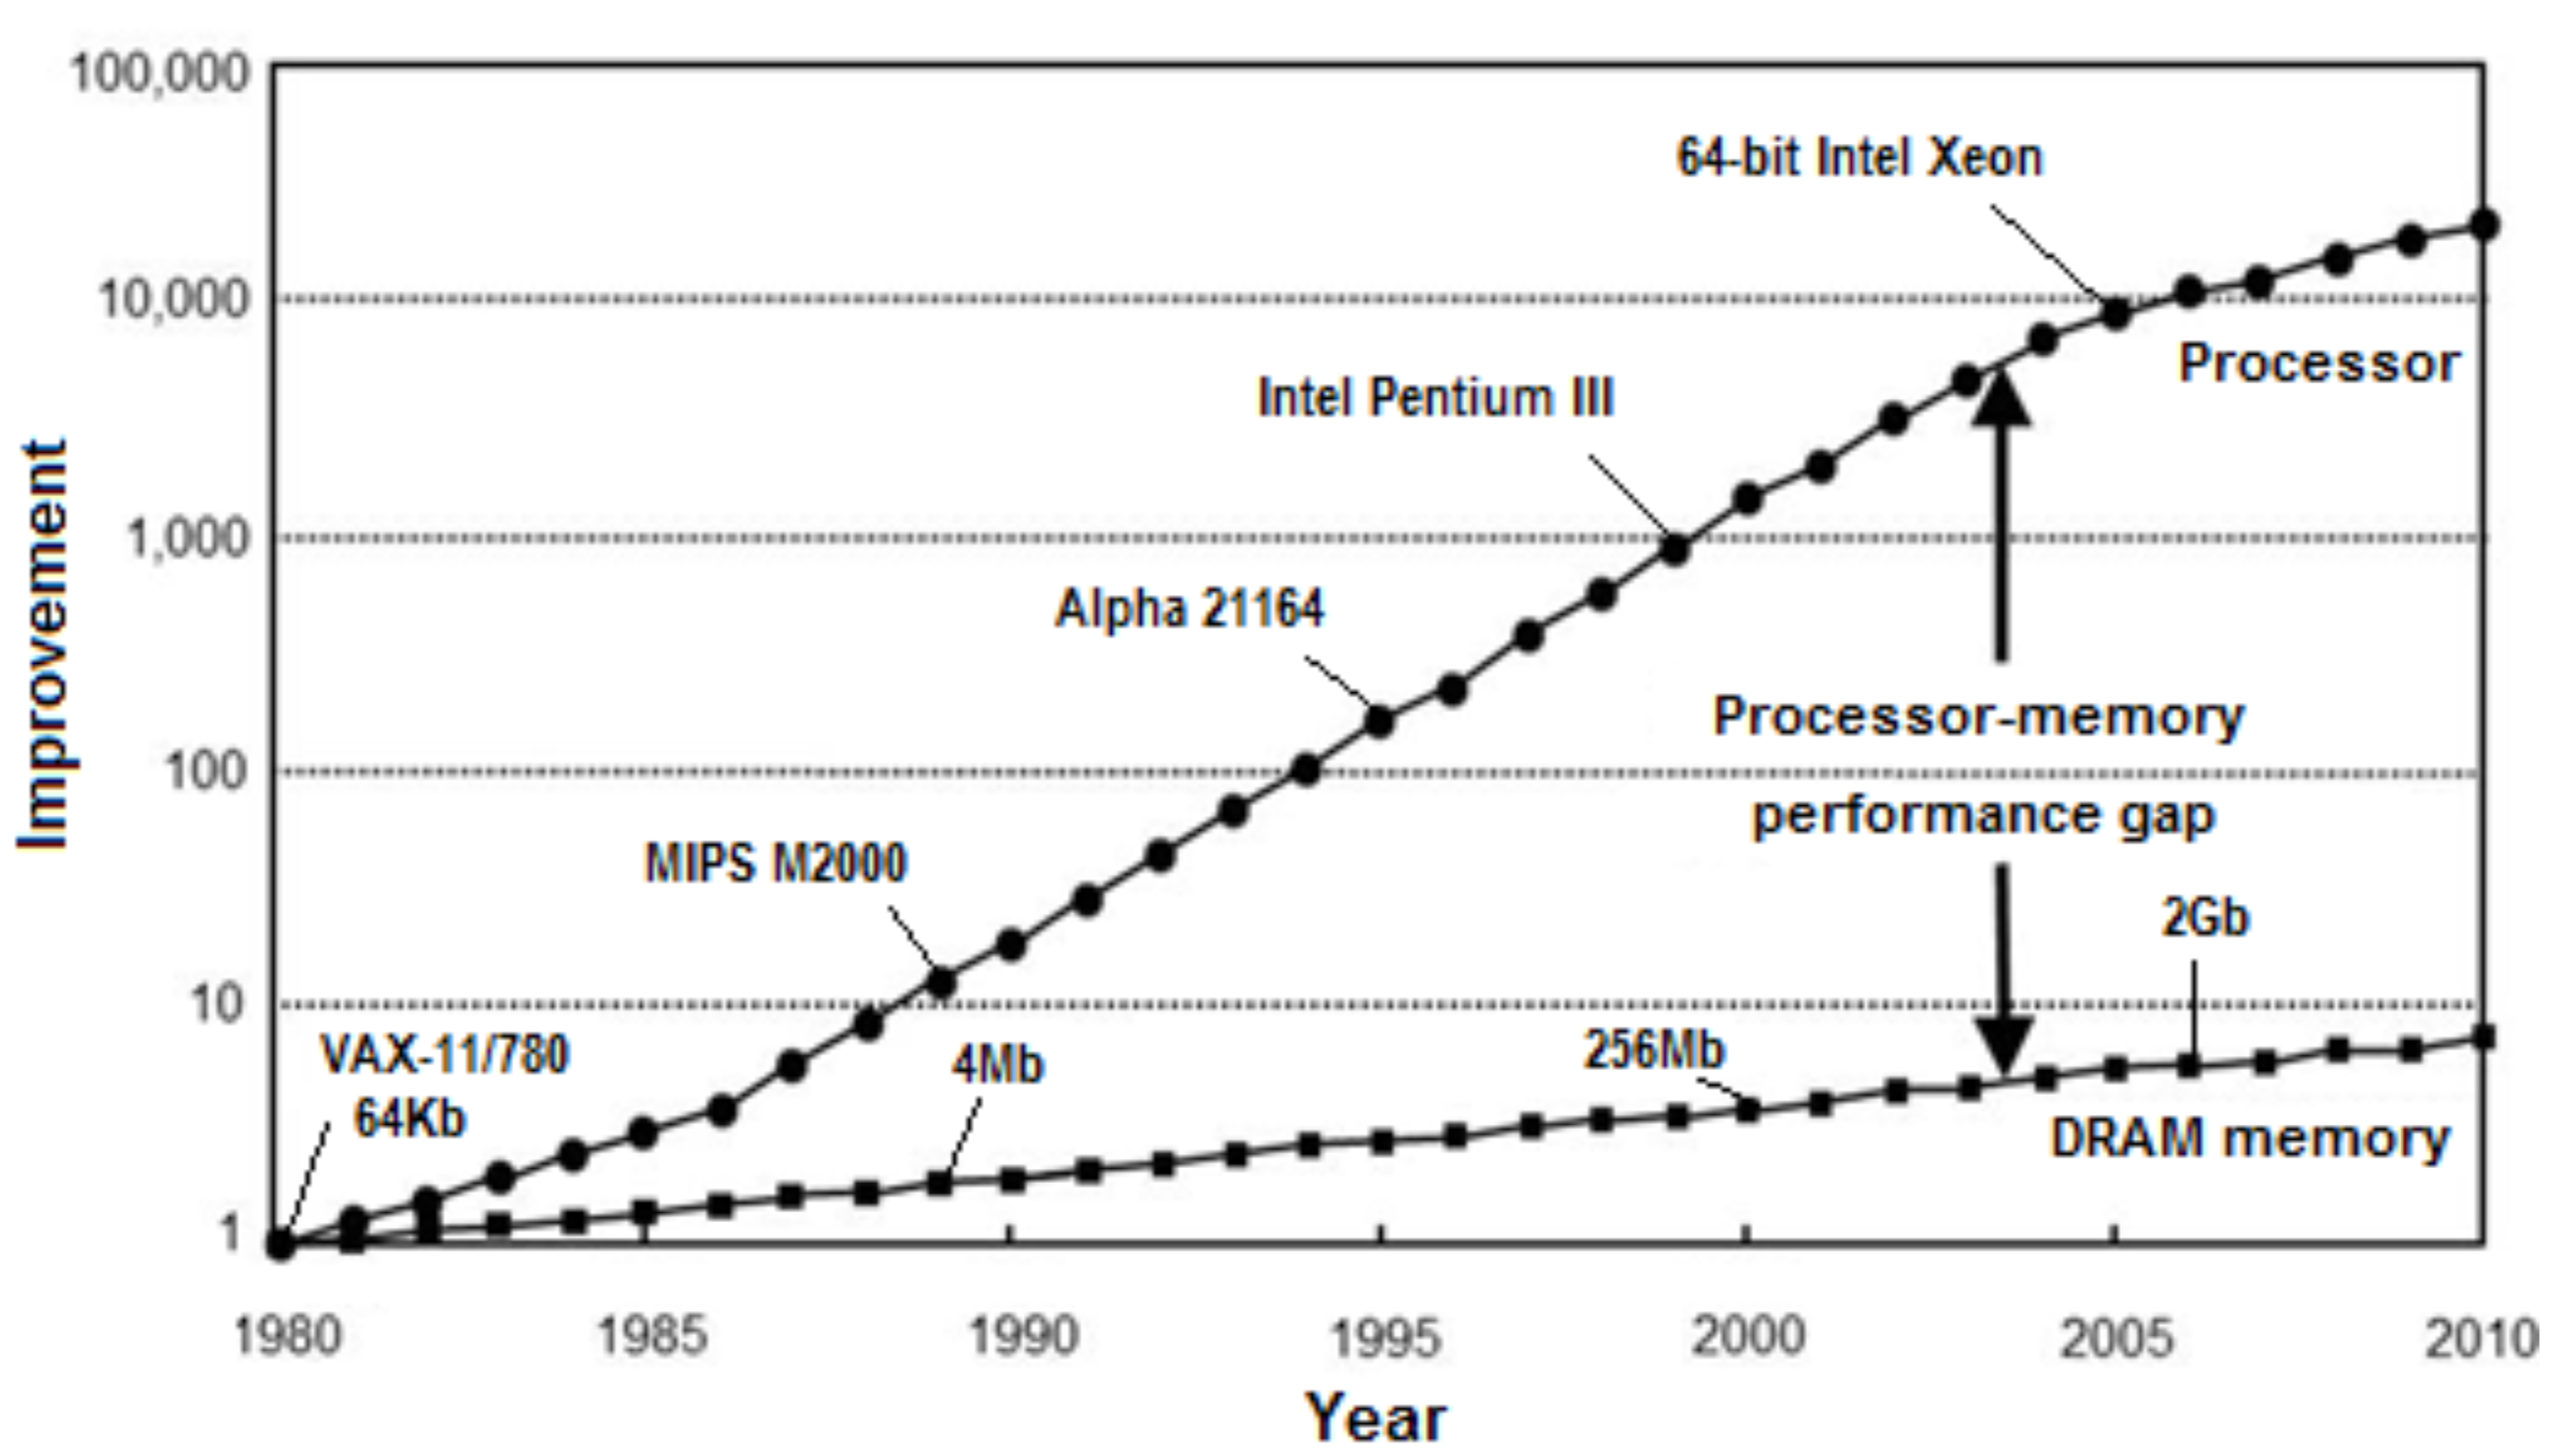
\includegraphics[width=10cm]{images/cpu_cpu_vs_memory.png}             \caption{\label{pic:cpuvsmemory2} Progression de la performance des processeurs et des mémoires. La performance de plusieurs générations de processeurs a été mesurée à l'aide du benchmark SPECint \cite{Efnusheva2017ASO}. La performance mémoire est représentée par la latence des accès mémoire (CAS et RAS) des mémoires DRAM.}
            \end{figure}
            
            Le déséquilibre des microarchitectures se fait d'autant plus ressentir lorsque des centaines de serveurs sont réunis. La \autoref{fig:unbalance_flop_io} montre l'évolution de la puissance des serveurs et du débit mémoire des 10 premiers supercalculateurs du Top500. Grâce aux évolutions des processeurs (voir \autoref{sec:proc_evo_2012}) et l'utilisation des GPUs, la puissance des serveurs a été multipliée en moyenne par 65 entre 2010 et 2018 (courbe bleue). Pendant la même période, le débit des communications interserveur n'a lui augmenté que d'un facteur 4.8 (courbe rouge). Ainsi, le ratio entre la puissance de calcul des serveurs et le débit de communication (byte par \gls{FLOP}) n'a fait que diminuer. Entre 2017 et 2018, ce ratio a diminué d'un facteur 8 pour les 2 premiers supercalculateurs du Top500 (respectivement Sunway Taihulight et Summit). Pour des applications nécessitant de grandes communications interserveur, ce ratio très faible les empêche d'atteindre plus d’une fraction de la performance disponible.
            
            \begin{figure}             \center             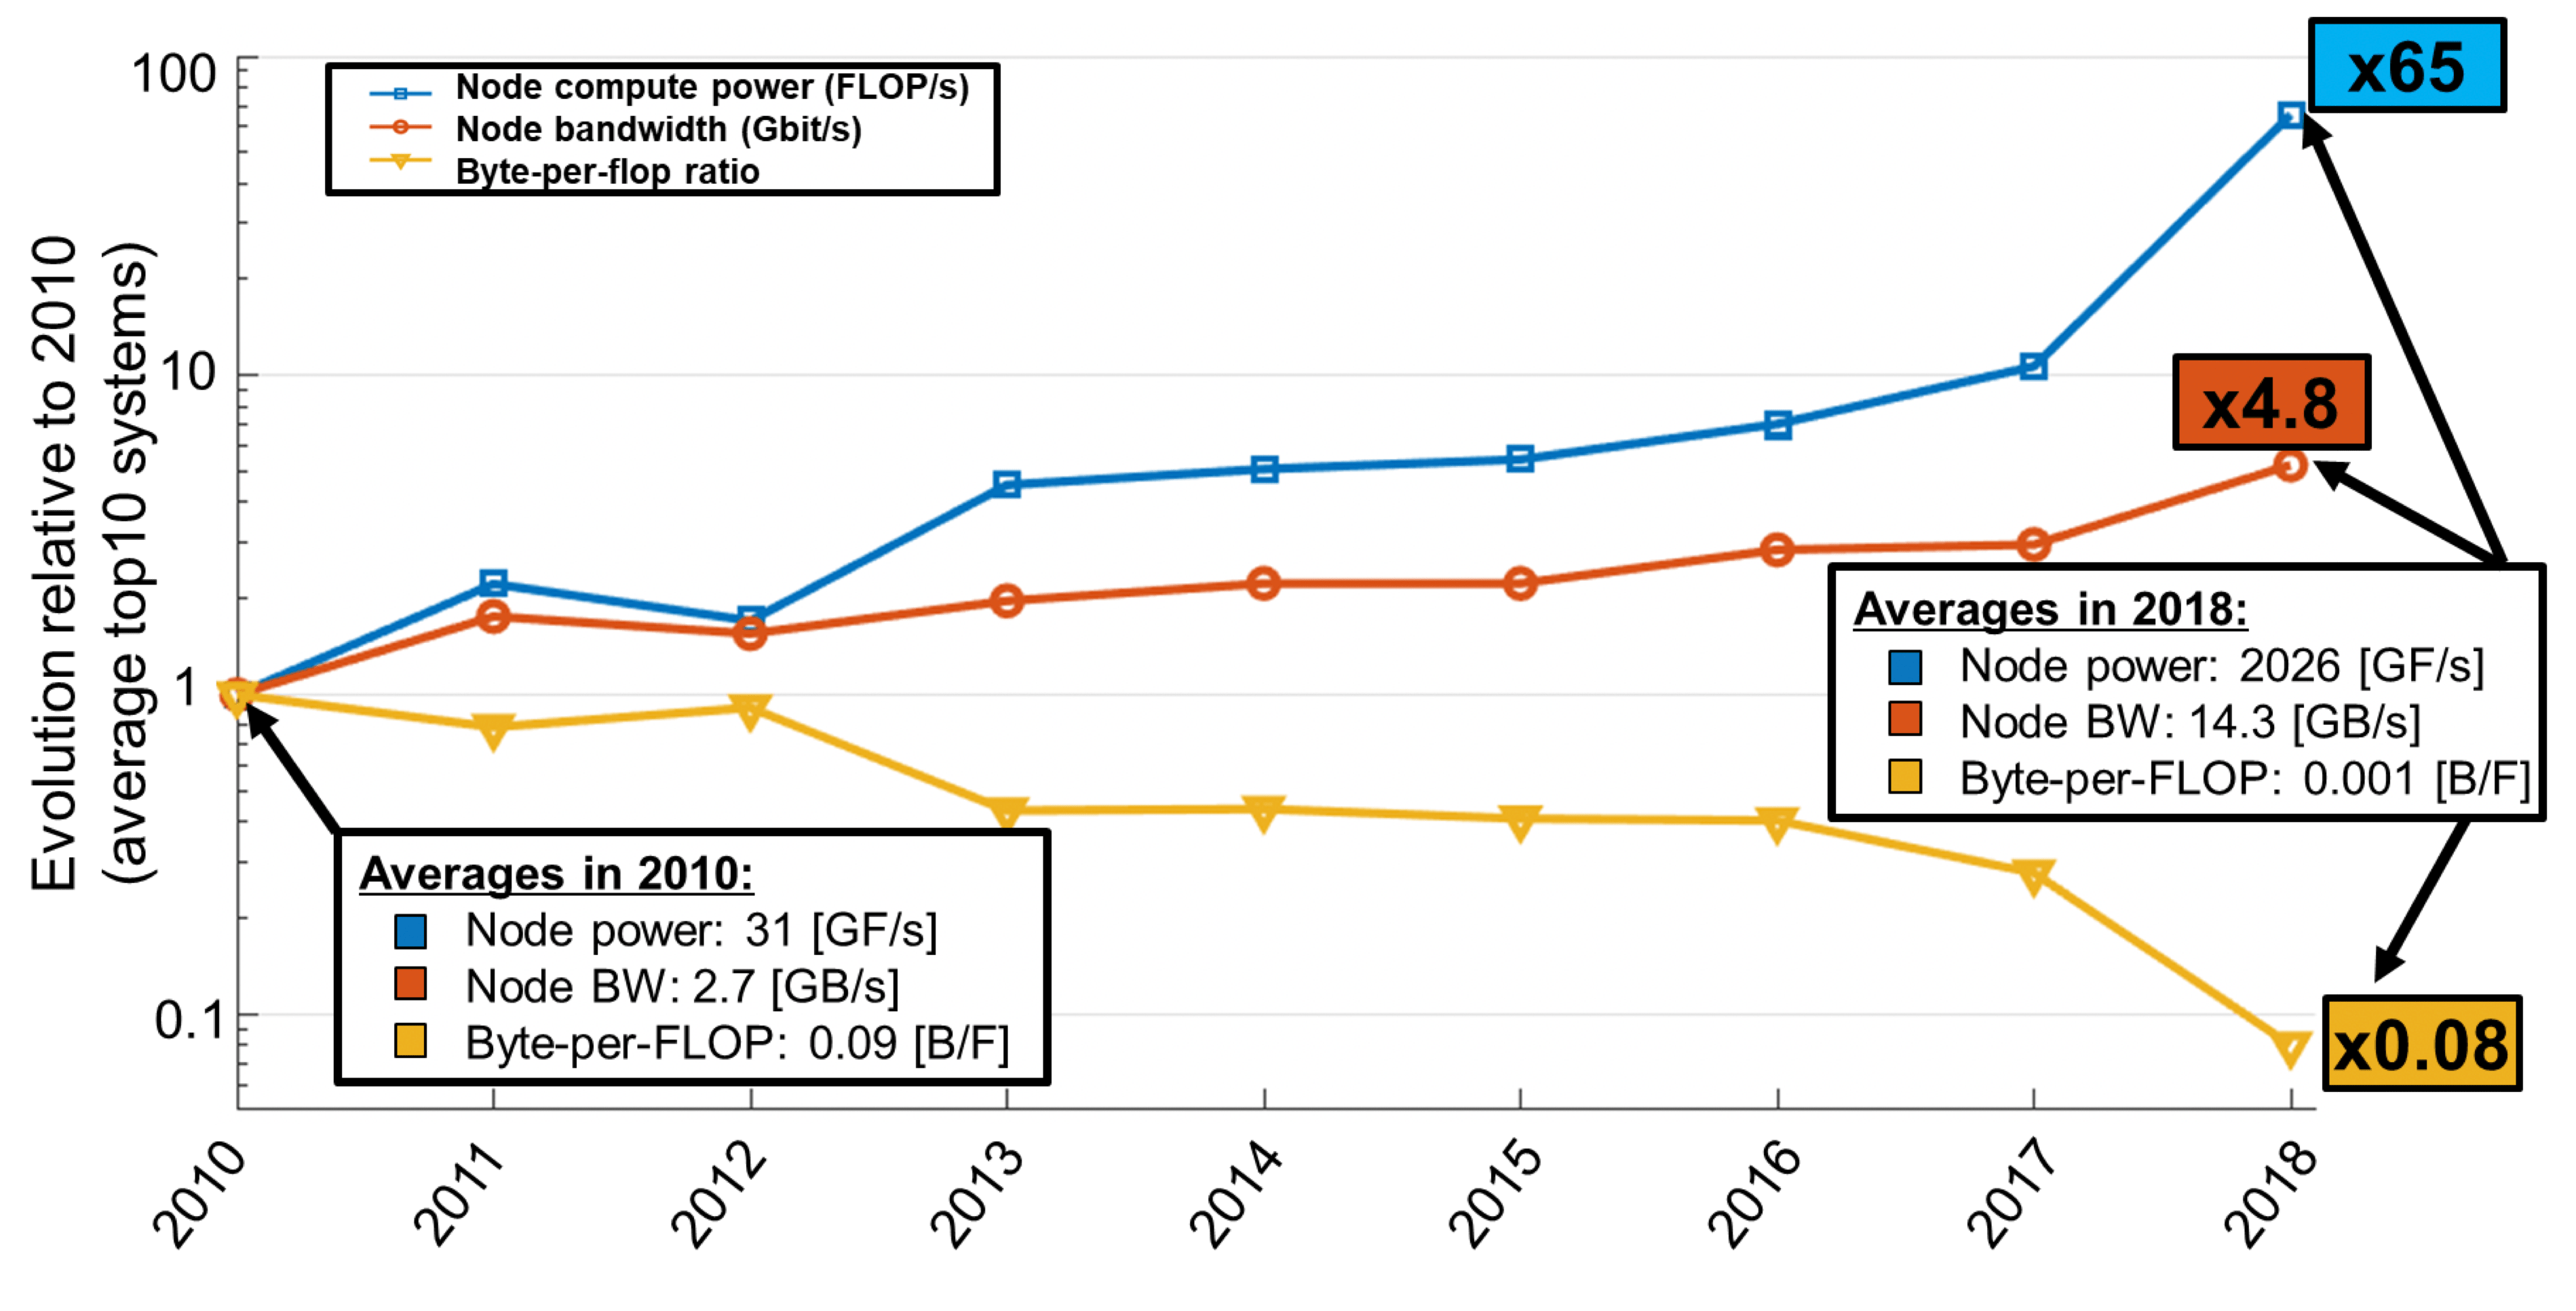
\includegraphics[width=12cm]{images/unbalance_flop_io.png}             \caption{\label{fig:unbalance_flop_io}Évolution des 10 premiers supercalculateurs du Top500 de 2010 à 2018: la puissance de calcul des serveurs (FLOP/s) en bleu, le débit de communication entre les serveurs (Gbit/s) en orange, ainsi que le ratio entre ces deux caractéristiques (byte par \gls{FLOP}) en jaune. (graphique tiré de la conférence IPDPS 2018 \cite{Bergman2018})}             \end{figure}
 
 
\subsection{Le futur du HPC}
%%%%%%%%%%%%%%%%%%%%%%%%%%%%%%%%%%%%%%%%%%%%%%%%%%%%%%%%%%%%%%%%%%%%%%%%


    \begin{fancyquotes}
    Peu importe la puissance qu'atteindront les processeurs, le logiciel trouvera toujours une façon d'utiliser cette puissance. Construisez un processeur 10 fois plus rapide, et la partie logiciel trouvera toujours 10 fois plus à faire (ou le fera 10 fois moins efficacement)  \cite{Sutter2005a}.
    \end{fancyquotes}
 
    \subsubsection{Situation du HPC en 2020}
    %%%%%%%%%%%%%%%%%%%%%%%%%%%%%%%%%%%%%%%%%%%%%%%%%%%%%%%%%%%%%%%%%%%%%%%%

   
        %EVO DES PERFORMANCES IT
        
        La performance des supercalculateurs et des technologies de l'information n'a fait qu'augmenter au cours de ces 30 dernières années. Une montre connectée récente apporte une puissance de calcul deux fois supérieure à celle du supercalculateur Cray-2, le plus puissant des supercalculateurs de 1985. Un GPU moderne tel que le GPU Nvidia V100 délivrant une puissante de 7.5 téraFLOPS ($10^{12}$ \gls{FLOPS}) serait classé à la 30e place du Top500 de 1994.

        %HPC: PLUS QUE DU CALCUL, UN MODE DE VIE
        L'évolution des performances des matériels informatiques a largement transformé le mode de vie de nos sociétés. Les produits du HPC sont présents dans nos vies quotidiennes que ce soit lorsque nous nous déplaçons grâce à l'essence extraite à l'aide de la modélisation des fonds marins ou lorsque nous consultons la météo. Le HPC a un réel impacte sur nos vies, les rendant plus sécurisées en prévoyant précisément des catastrophes naturelles. 

        %IL Y A UNE DEMANDE DE PLUS DE CALCUL
  
        Suite à la forte évolution de la performance des supercalculateurs, nous pouvons nous demander s'il est nécessaire de continuer à construire des infrastructures toujours plus puissantes. La variété et la complexité des problèmes qui peuvent être traités dépendent directement de la puissance de calcul disponible. L’apprentissage profond (\textit{deep learning}) en est un bon exemple. Dès 1989, Yann LeCun améliorait déjà la rétropropagation \cite{Treibig2012a} et utilisait les réseaux neuronaux convolutionnels \cite{LeCun1989}. Mais à cette époque les GPGPU n'étaient pas disponibles et les CPU étaient loin d'être assez puissants pour exécuter ces algorithmes, même sur les données limitées disponibles à cette époque. Dans les années 2010, les GPU sont devenus suffisamment puissants pour permettre l'exécution de ces algorithmes.
        
        
        La mise au point de plateformes plus puissantes va permettre aux entreprises d'être plus compétitives et aux équipes de recherches de réaliser de nouvelles découvertes. Un grand nombre de domaines scientifiques vont pouvoir profiter de telles puissances de calcul: découverte de nouveaux matériaux, simulations de réactions chimiques ou encore pour analyser les résultats d'expériences lourdes comme celles réalisées au Grand collisionneur de hadrons \cite{10.1007/978-3-319-67630-2_52}. La recherche pour le climat va aussi bénéficier de telles architectures et permettre de comprendre les dérèglements climatiques, anticiper la hausse des océans et élaborer de meilleurs modèles. Les simulations permettront également d'améliorer l'efficacité et la sécurité des réacteurs nucléaires \cite{Simon2007}. En astrophysique, elles permettront d'étudier des phénomènes encore incompris comme la formation des trous noirs \cite{10.1007/978-3-642-38750-0_2}. L'accès à des infrastructures plus puissantes permettra de poursuivre les avancées réalisées dans le domaine de la physique quantique. Ces découvertes pourront permettre de construire d'autres plateformes de calculs appelées ordinateurs quantiques.
        
         
    \subsubsection{Nécessité de construire des plateformes plus puissantes}\label{sec:3_motivations}
    %%%%%%%%%%%%%%%%%%%%%%%%%%%%%%%%%%%%%%%%%%%%%%%%%%%%%%%%%%%%%%%%%%%%%%%%

        \begin{fancyquotes}
        La taille des données double tous les deux ans, et d'ici 2020, les données que nous générons et copions annuellement atteindront 44 Zettabytes ($10^{21}$ bytes) \cite{Zhang2017}.
        \end{fancyquotes}
    
        Aujourd'hui, de nombreuses applications sont prêtes, mais ne peuvent pas être exécutées en un temps raisonnable avec les moyens de calculs disponibles. Actuellement il est possible de simuler des réactions chimiques de quelques nanosecondes et sur de petits volumes. Avec la construction de supercalculateurs plus puissants, il sera possible de réaliser des simulations plus longues et plus précises. Nous discutons dans cette section de trois facteurs importants qui motivent la nécessité de poursuivre le développement de plateformes plus performantes que celles actuellement en notre possession: l'explosion du volume de données à traiter, la complexification des analyses et le besoin d'obtenir des résultats rapidement.

        
        \paragraph{Tsunami de données.} 
            
            Suite aux évolutions des technologies des semi-conducteurs, nous assistons depuis le début des années 2010 à l'explosion des quantités de données générées (voir \autoref{fig_edl_bigdata}). Grâce aux nanotechnologies, il est possible de produire des capteurs à très faible coût. La consommation électrique de ces matériels étant faible, ces capteurs sont installés partout. L’Internet des Objets (IOT) interconnecte ces milliers de capteurs pour générer de grands volumes de données (\textit{big data}).  Les évolutions récentes de la domotique ont permis d'installer des capteurs dans toute la maison: que ce soit pour gérer les lumières, le chauffage, l'ouverture des volets ou même l'allumage de la cafetière. En 2018, Ericsson comptait plus de 5 milliards d'abonnés au téléphone dans le monde\footnote{Source: \url{https://www.usinenouvelle.com/article/5-4-milliards-d-abonnes-au-telephone-mobile-dans-le-monde.N739439}}. Ces téléphones peuvent aujourd'hui suivre nos moindres faits et gestes, générant de grandes quantités de données. Celles-ci peuvent ensuite être utilisées par différentes applications pour étudier les déplacements des habitants d'une ville ou proposer des annonces ciblées. Les villes installent des milliers de capteurs permettant le développement de nombreuses applications comme le suivi du trafic routier \cite{bonhomme:hal-01334670}, l'optimisation des transports en commun, ou encore le suivi du recyclage des déchets dans un quartier \cite{Rebelles2018}. Ce grand volume de données produit aujourd'hui et qui va s'intensifier dans les années futures est le principal défi des systèmes d'informations.
        
              
            \begin{figure}
            \center
            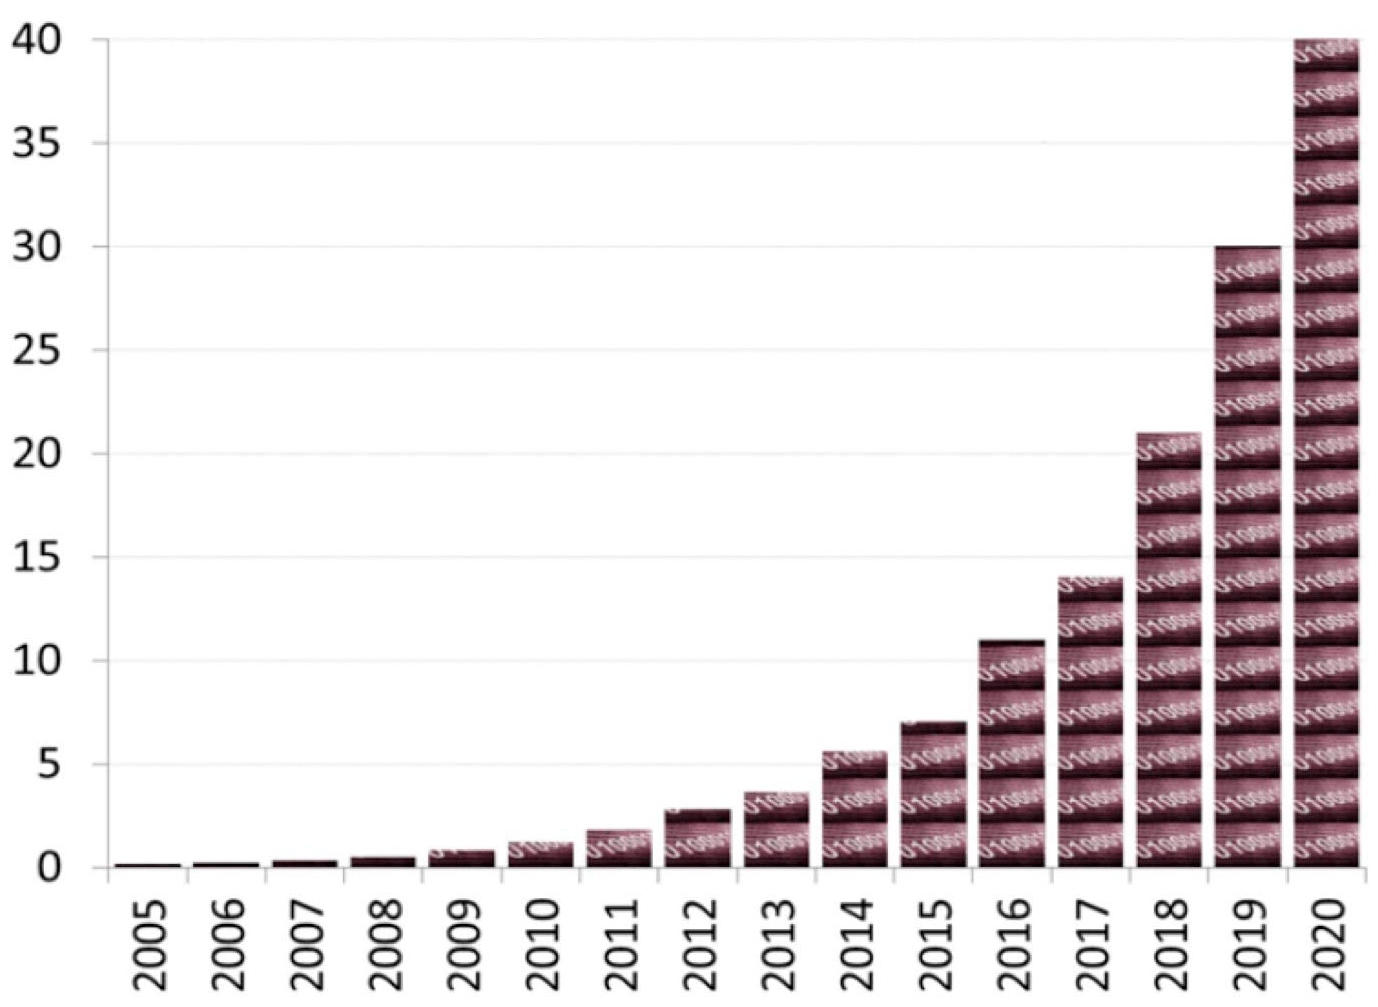
\includegraphics[width=10cm]{images/edl_bigdata.png}
            \caption{\label{fig_edl_bigdata} Le volume de données généré chaque année devrait atteindre 40 Zettabytes en 2020 \cite{Simoudis2016}}
            \end{figure}
        
        

            
        \paragraph{Complexité des calcus.} 
             Aujourd'hui, la valeur ne provient plus de la capacité à produire ces données, mais de la capacité d'en extraire une valeur avec des algorithmes de \textit{big data} et d'apprentissage machine. Les algorithmes d'intelligence artificielle nécessitent d'être entraînés sur des jeux de données pour pouvoir ensuite prendre les décisions adaptées. En 2018, OpenAI a constaté que la puissance de calcul utilisée pour entraîner les plus grands modèles d'IA avait doublé tous les 3,4 mois depuis 2012 (voir \autoref{fig_edl_ai_compute}). Dans le domaine de la santé, de telles infrastructures pourront permettre d'extraire et analyser toutes les informations de millions de patients atteints de maladies graves.  Il sera alors possible de mieux comprendre les symptômes menant au développement d'un cancer ou d'une maladie cardiaque. 
             Pour obtenir des résultats dans des temps raisonnables, ces applications nécessitent d'avoir accès à des plateformes plus puissantes de plusieurs facteurs que celles existant actuellement. Avec l'analyse des données obtenues grâce aux montres connectées, il sera alors possible d'anticiper les maladies cardiaques.
             
            \begin{figure}
            \center
            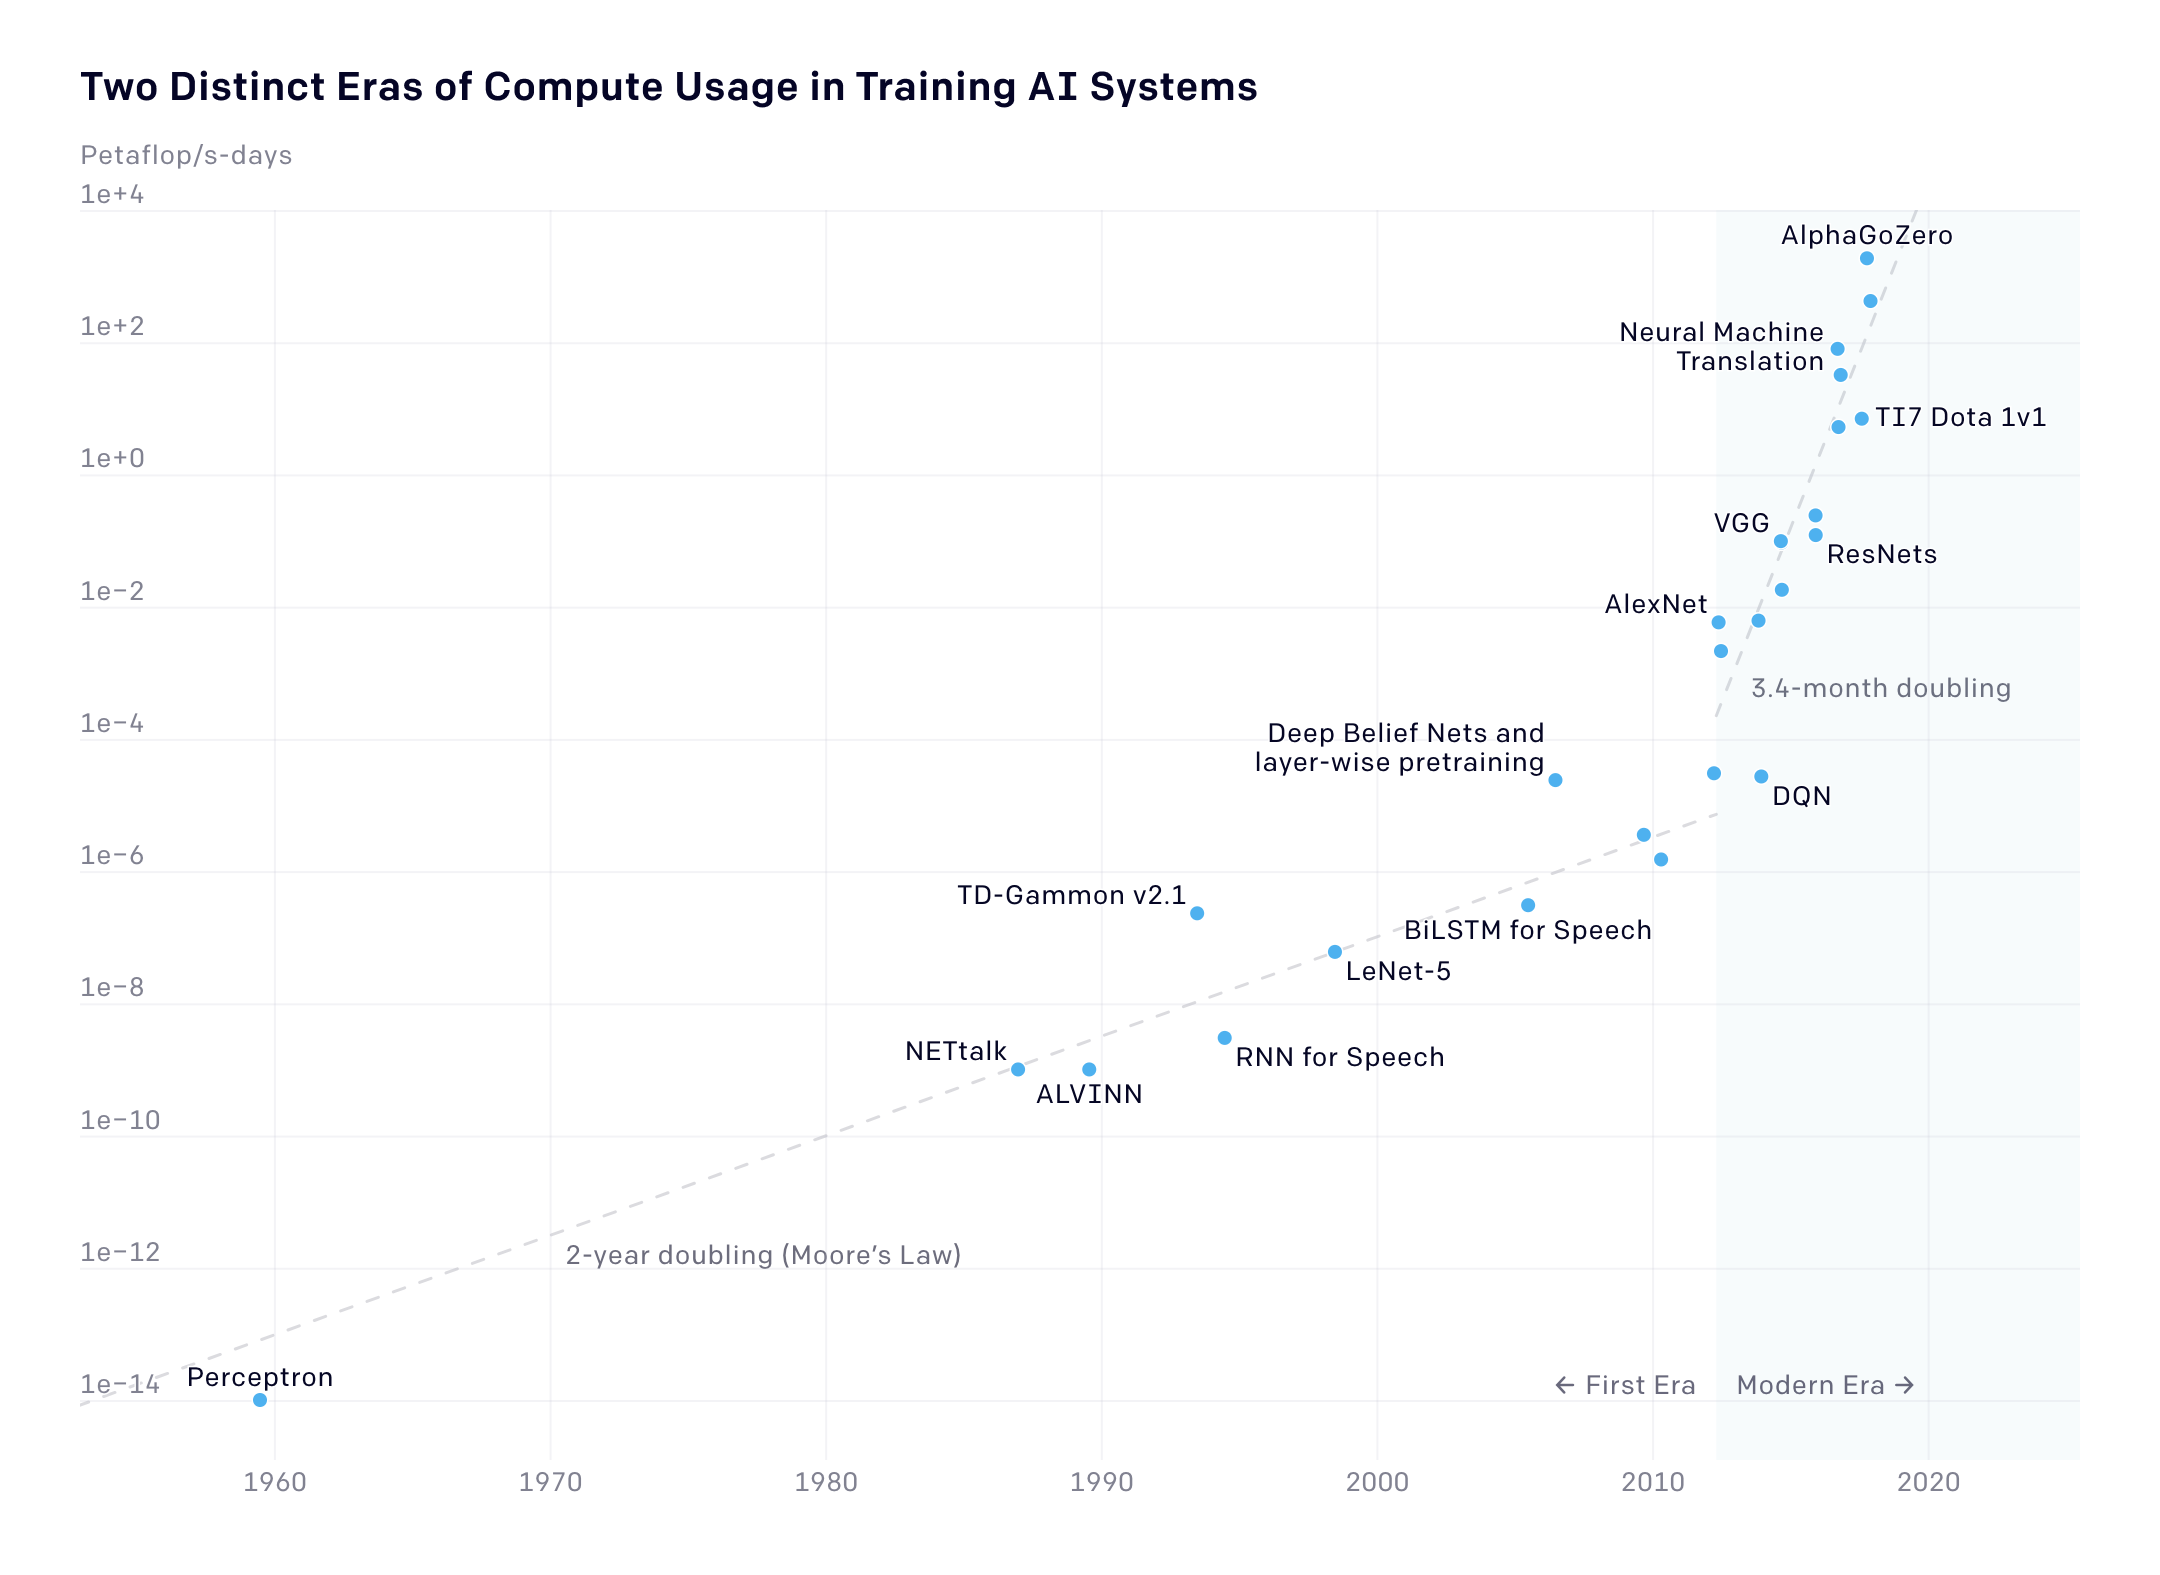
\includegraphics[width=14cm]{images/edl_ai_compute.png}
            \caption{\label{fig_edl_ai_compute} Quantité totale de calcul (en pétaFLOPS ($10^{15}$ \gls{FLOPS})) nécessaire chaque jour pour entraîner les différents réseaux de neurones \cite{amodei2ai}.}
            \end{figure}

        \paragraph{Temps de traitement.} 
        
            La troisième raison qui motive le développement de nouvelles plateformes plus puissantes est de réduire le temps d'exécution des applications. Une fois la donnée produite, sa valorisation diminue dans le temps. La météo est un très bon exemple d'application ne pouvant pas excéder un certain temps de traitement si les prédictions veulent être données suffisamment rapidement. Par exemple, pour permettre aux voitures connectées d'identifier un danger, l'action correspondante doit être prise le plus rapidement possible. La possibilité d'envoyer les données à traiter à un supercalculateur n'est alors pas envisageable. L'accès à des plateformes plus puissantes est alors nécessaire pour traiter cette quantité de données dans des temps raisonnables. En plus d'améliorer les performances des supercalculateurs, l'architecture complète des plateformes doit être repensée. Pour traiter efficacement le volume de données générées, plusieurs travaux montrent qu'il est indispensable de repenser notre façon de stocker, déplacer et analyser ces données \cite{Saltz2018, Chen2014, Nahrstedt2017, GeoffreyFoxJhaShantenu2015}.
  
 
    \subsubsection{Exascale}\label{sec:exascale}
    %%%%%%%%%%%%%%%%%%%%%%%%%%%%%%%%%%%%%%%%%%%%%%%%%%%%%%%%%%%%%%%%%%%%%%%%
        
      
        %Exascale Definition maison             
        
        Le terme \gls{exascale} est utilisé pour définir la prochaine génération de supercalculateurs capable d'atteindre une performance de \gls{exaFLOPS}. Cette performance devra être mesurée à l'aide du benchmark High-Performance Linpack (HPL \cite{Dongarra2003}). En effet, certains supercalculateurs sont déjà capables d'atteindre de telles performances sur des applications plus simples. En 2018 le supercalculateur Summit était capable d'exécuter $1.2 * 10^{18}$ opérations par seconde. L'application utilisée était une application d'apprentissage en profondeur utilisée pour étudier les déchets nucléaires.  Cette application n'utilise que des opérations en simple précision. Le même supercalculateur a pu atteindre une performance de $3.3 \times 10^{18}$ opérations sur une application d'analyse de données, elle aussi en simple précision \cite{Bergman2018}.
         \footnote{\url{https://insidehpc.com/2019/11/deep-learning-on-summit-supercomputer-powers-insights-for-nuclear-waste-remediation/}}. 
        
        Dans la littérature, il est courant d'utiliser le terme \textit{exascale} pour désigner cette nouvelle génération de plateformes 10 fois plus puissantes que les supercalculateurs les plus puissants actuels, et 30 fois plus puissants que la moyenne du Top500 de novembre 2019 (33 pétaFLOPS). Le rapport commandé par le département de l'énergie américain en 2014 \cite{Lucas2014} souligne que ce terme ne fait pas référence à la puissance obtenue par le benchmark HPL, mais bien à une plateforme avec 1000 fois plus de capacité que les supercalculateurs existant alors. Dans ces travaux de thèse, nous suivons la même démarche et utilisons le terme exascale pour désigner la plateforme qui permettra d'obtenir les performances souhaitées. La plateforme ne concerne pas seulement le supercalculateur, mais toute la chaîne de traitement de données, depuis sa création jusqu'à son traitement.


\subsection{Défis à relever pour l'élaboration d'une plateforme exascale} \label{sec:challenges}
%%%%%%%%%%%%%%%%%%%%%%%%%%%%%%%%%%%%%%%%%%%%%%%%%%%%%%%%%%%%%%%%%%%%%%%%

    %La course à peta etait dure
        
    Jusqu'aujourd'hui, quand une piste d'évolution venait à s'épuiser, comme l'évolution de la fréquence des processeurs, d'autres améliorations venaient alors y pallier (augmentation du nombre de coeurs). Dans la \autoref{sec:Top500}, nous avons discuté des principaux freins ayant ralenti l'évolution des performances des supercalculateurs ces 8 dernières années. Depuis plusieurs années, de nombreuses études \cite{Shalf2010, bergman2008exascale, Bergman2011} prédisent les principaux challenges à relever pour la construction d'une plateforme exascale. La plus citée d'entre elles est l'étude menée par le département de l'énergie américain \cite{Lucas2014} qui décrit les dix principaux challenges à relever. Ce rapport met en lumière les nombreuses difficultés que l'industrie rencontre et montre que celles-ci touchent toutes les parties des centres de données (\textit{data center)}): l'énergie, les technologies mémoire et d'interconnexion, la programmation, la gestion ou encore la capacité des applications à utiliser la totalité de la puissance disponible. 
    Il est aussi indiqué que pour construire une telle plateforme dans des coûts financiers et des consommations électriques raisonnables, les dernières avancées technologiques des domaines cités précédemment doivent être intégrées. Le travail de la thèse a en partie été motivé par ces challenges présentés dans les études citées ci-dessus. Dans cette section nous présentons en détail les six principales difficultés que nous avons identifiées. 

    \subsubsection{Les coûts}\label{sec:edl_chal_prix}
    %%%%%%%%%%%%%%%%%%%%%%%%%%%%%%%%%%%%%%%%%%%%%%%%%%%%%%%%%%%%%%%%%%%%%%%%
    %%%%%%%%%%%%%%%%%%%%%%%%%%%%%%%%%%%%%%%%%%%%%%%%%%%%%%%%%%%%%%%%%%%%%%%%

    %MOORE et Transistor $
    
        Dans la \autoref{sec:end_mooore} nous avons expliqué comment la fin de la loi de Moore avait impacté l'évolution des performances des supercalculateurs. Bien que souvent oubliée, il est important de rappeler que cette loi est avant tout une loi économique.
        Grâce à l'évolution des procédés de gravure, le nombre de transistors a pu doubler tous les deux ans pendant plus de trente ans alors que le coût des investissements dans les fonderies n'augmentait que de 30\% sur la même période. Cette évolution des prix des fonderies porte le nom de \textit{seconde loi de Moore} ou loi de Rock. À cause des nombreux investissements nécessaires pour développer les nouvelles générations de fonderies nous remarquons que le nombre de transistors achetable pour un budget donné n'évolue plus (voir \autoref{fig:edl_moore_dollars}).
    
        \begin{figure}
        \center
        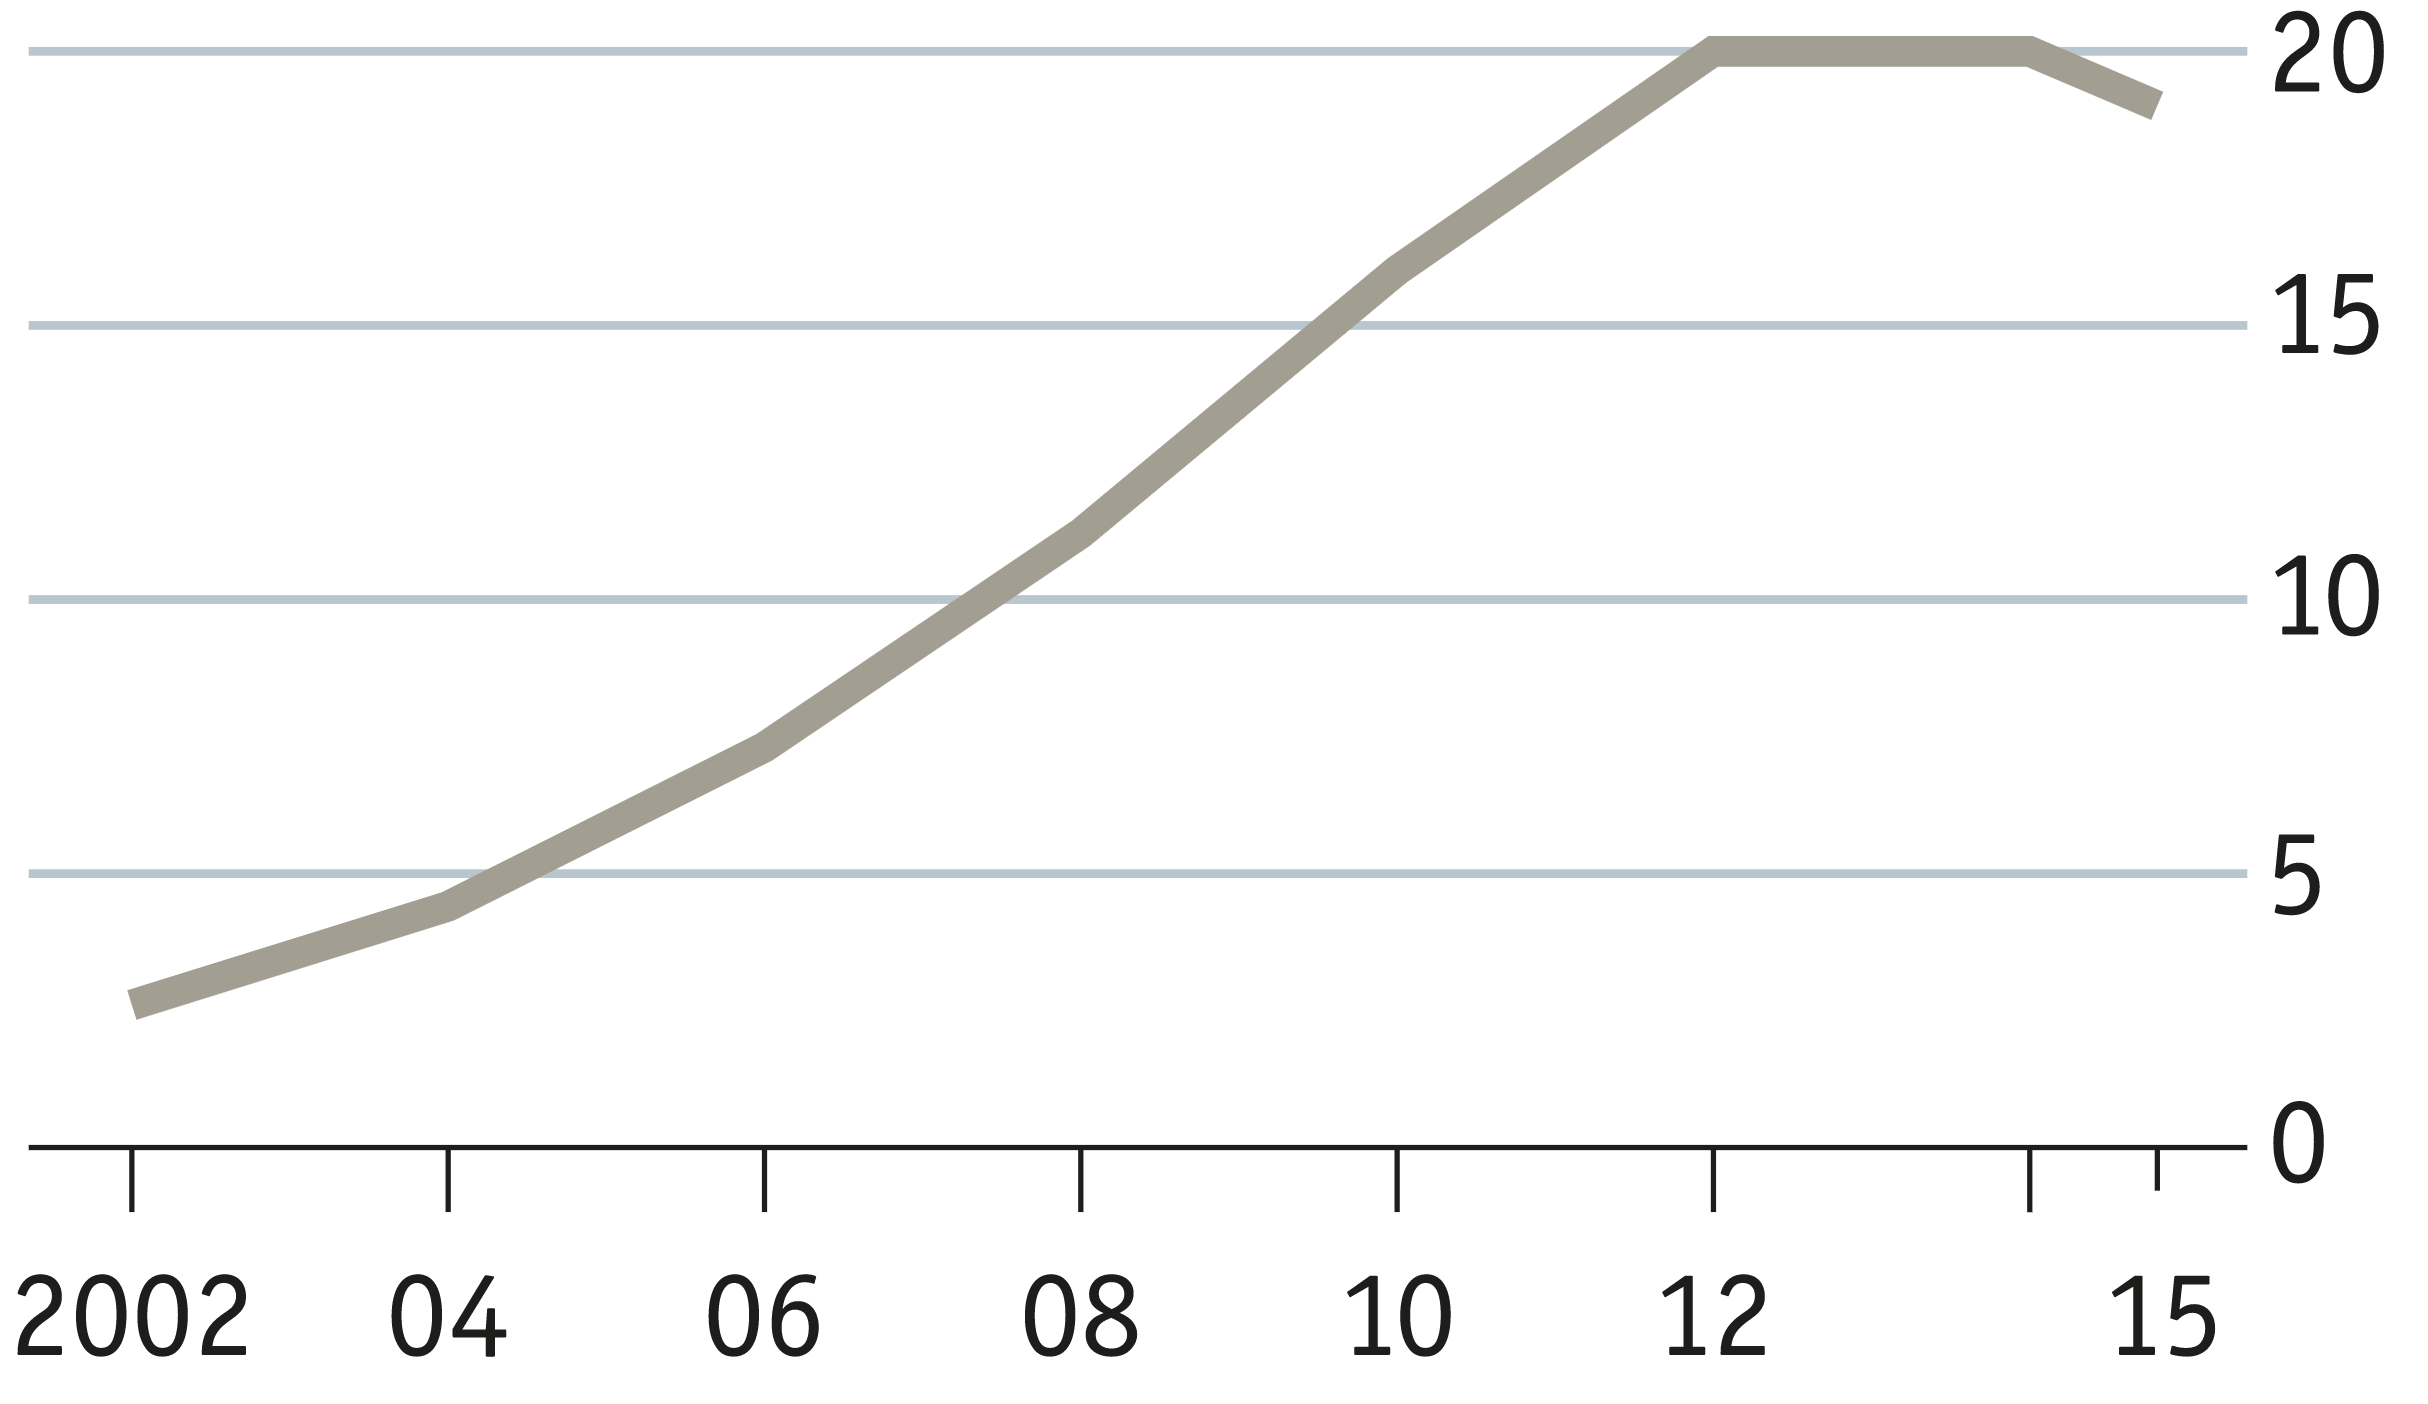
\includegraphics[width=8cm]{images/edl_moore_dollars.png}
        \caption{\label{fig:edl_moore_dollars} Nombre de transistors achetés par dollar dépensé\protect\footnotemark.}
        \end{figure}
        \footnotetext{Source: Intel ; rapport de presse ; Bob Colwell ; Linley Group; The Economist ; IB Consulting}

  %Data center
    

        Le prix d'un supercalculateur n'est pas seulement constitué de l'addition du prix des processeurs et des mémoires. Elle prend en compte le Coût Globale de Possession (TCO) (voir \autoref{sec:methodo_step4}). Cette valeur prend en compte le cumul des coûts du centre de données durant la totalité de son cycle de vie. Il tient compte du prix du bâtiment dans lequel se trouve le supercalculateur, de sa consommation électrique, mais aussi de l'opérationnel (personnel nécessaire pour sa gestion). Tous ces facteurs doivent être pris en compte, le prix de l'électricité tenant une grande part dans l'équation. 
        Pour les entreprises, le facteur économique est souvent le premier critère de décision. Les budgets alloués au développement et à l'utilisation d'une nouvelle plateforme sont décidés en amont et il est rare que des budgets supplémentaires soient alloués, même pour une plateforme plus performante. Lorsque HPE répond à des appels d'offres pour la construction d'un nouveau supercalculateur, les métriques utilisées sont les $FLOPS/\$$ ou $GB/s/\$$. Cette forte pression économique est une contrainte et il est difficile de proposer des sauts technologiques qui nécessitent de lourds investissements en amont sans connaître les retombées à l'avance. Lorsqu'une entreprise investit dans une solution, elle veut pouvoir quantifier à l'avance les bénéfices qu'elle peut en tirer. Lors de l'analyse du Top500, nous avons remarqué que la vitesse de l'accroissement des performances des supercalculateurs des entités avec les plus petits budgets avait ralenti 4 ans (2008) avant le reste du Top500 (2012). 
    
        
    \subsubsection{La consommation énergétique}\label{sec:edl_chal_energie}
    %%%%%%%%%%%%%%%%%%%%%%%%%%%%%%%%%%%%%%%%%%%%%%%%%%%%%%%%%%%%%%%%%%%%%%%%
    %%%%%%%%%%%%%%%%%%%%%%%%%%%%%%%%%%%%%%%%%%%%%%%%%%%%%%%%%%%%%%%%%%%%%%%%
  
        L'investissement dans un supercalculateur ne concerne pas seulement son acquisition. Un budget conséquent doit être alloué à l'alimentation du matériel, mais aussi du système de refroidissement. L’évolution de la consommation des processeurs a nécessité le développement de systèmes de refroidissement ultra-optimisés. Toute l’énergie étant transformée en chaleur, des techniques telles que le refroidissement à l’eau et l’immersion dans des bains d’huile sont régulièrement utilisées. Si on regarde la consommation électrique des clusters du Top500, on constate qu'en moyenne ils consomment 1,4 mégawatt et que les 5 qui consomment le plus sont au-delà de 12 mégawatts (voir graphique \ref{pic_top500_power}). En supposant que le prix de l'électricité coûte 1 dollar par watt par année, l'alimentation de ces architectures coûte alors annuellement des millions de dollars (20 millions de dollars pour le premier).
        
        En plus du coût financier, il est important de considérer l'impact écologique de la consommation électrique de ces plateformes. Une étude a été menée pour évaluer l’évolution de l’entraînement des principaux réseaux de neurones (AlexNet, AlphaGo, GoogleNet…) \cite{strubell-etal-2019-energy}. La quantité de calculs nécessaire pour l’entraînement d’un réseau a été multipliée par 300 000 en 7 ans. L’étude rapporte l’empreinte carbone de l’entraînement de ces réseaux. Le $CO_2$ émis lors de l'entraînement d’un réseau équivaut au $CO_2$ émis par un passager réalisant 300 allers-retours en avion entre New York et San Francisco ou encore à l’émission de cinq voitures américaines durant toute leur durée de vie.
                
                \begin{figure}
                    \center
                    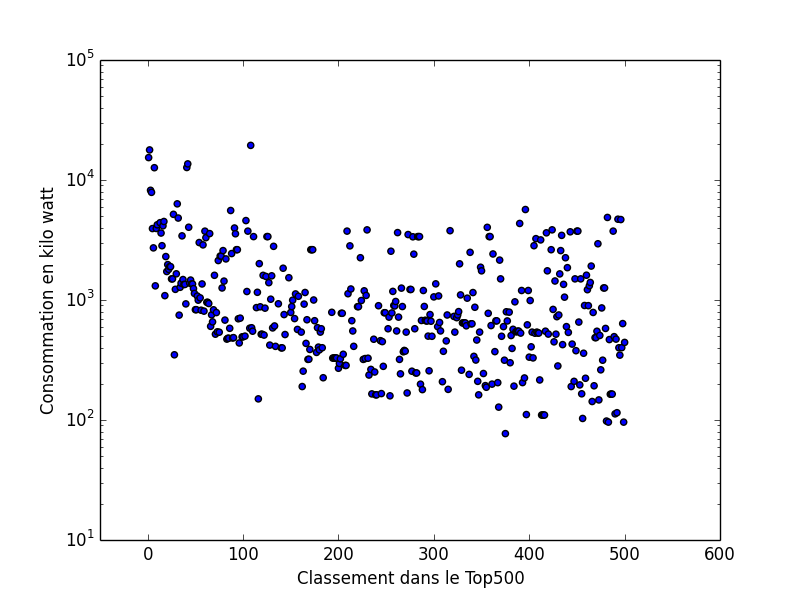
\includegraphics[width=10cm]{images/Chapitre1/pic_top500_power.png}
                    \caption{\label{pic_top500_power} Consommation électrique des 500 supercalculateurs les plus puissants (2018).}
                \end{figure}
      
      
        Le Département de l'énergie des États-Unis (DoE) a publié son rapport de propositions PathForward, et a établi qu'un supercalculateur exaflopique devra consommer au maximum entre 20 et 30 mégawatts \cite{Ang2016}. Actuellement, les quatre premiers supercalculateurs consomment entre 7 et 18 MW. La construction d'une plateforme exascale implique donc de réaliser 30 fois plus d'opérations avec une enveloppe énergétique seulement doublée. L'énergie est une contrainte majeure dans la construction d'une plateforme Exascale. Pour nous en rendre compte, nous étudions le dernier classement du Top500 paru en novembre 2019. Pour obtenir une puissance cumulée d'un exaFLOPS, il faut additionner la puissance des 105 premiers supercalculateurs du Top500. Une telle plateforme nécessiterait alors une alimentation de plusieurs centaines de mégawatts. Le même exercice peut être réalisé avec le classement du Green500 (voir \autoref{tab:green500}), qui classe les architectures les plus efficaces du Top500. Pour obtenir une puissance cumulée d'un exaFLOPS, il faudrait regrouper les 205 premiers supercalculateurs pour obtenir une plateforme consommant 279 MW. Ces rapides calculs permettent de montrer l'étendue vertigineuse des améliorations qui sont nécessaires pour la construction d'une plateforme qui respecterait les critères de consommation \cite{Ang2016}. 
        
        
        
        \paragraph{Consommation de la microarchitecture.} 
            
            Ajouter des serveurs pour la construction d'un supercalculateur plus puissant nécessite une plus grande puissance électrique. Cette technique est restée viable pendant plus de vingt ans, alors que les processeurs ne consommaient que quelques watts. Aujourd'hui, les processeurs utilisés ont une enveloppe thermique (TDP) dépassant la centaine de watts: 190 watts pour le processeur IBM Power9 22 coeurs (utilisé dans le supercalculateur Summit), 150 watts pour le processeur Intel Skylake 6148 20 coeurs (utilisé dans le 8e supercalculateur du classement du Top500 2019). Les plateformes les plus puissantes associent à un processeur un ou plusieurs accélérateurs (principalement des GPU). Chaque noeud du supercalculateur Summit possède ainsi 2 processeurs et 6 GPU NVidia V100 ayant chacun un TDP de 250 watts. À de telles consommations, il n'est plus viable d'ajouter des noeuds de calculs indéfiniment, que ce soit pour une raison de coût ou bien de faisabilité. En effet, les sites où sont construits les centres de données ont des lignes électriques déjà existantes et qui ne peuvent pas supporter de plus grandes puissances. Une partie des utilisateurs sont donc limités par cette enveloppe énergétique et doivent l'utiliser le plus efficacement pour la transformer en puissance de calcul. La consommation électrique des architectures varie fortement en fonction des opérations réalisées (voir \autoref{fig:energy_pj}). Que ce soit pour des architectures 32 bits \cite{Horowitz2014} ou 64 bits \cite{Leland2014} la consommation électrique des opérations élémentaires de la microarchitecture n’a que très peu évolué ces dernières années. Nous constatons que la majorité du budget énergétique est allouée au déplacement des données entre la mémoire et les caches. Il est donc primordial d'apporter des solutions matérielles et logicielles permettant de réduire la consommation de ces opérations.
        
            \begin{figure}
            \center
            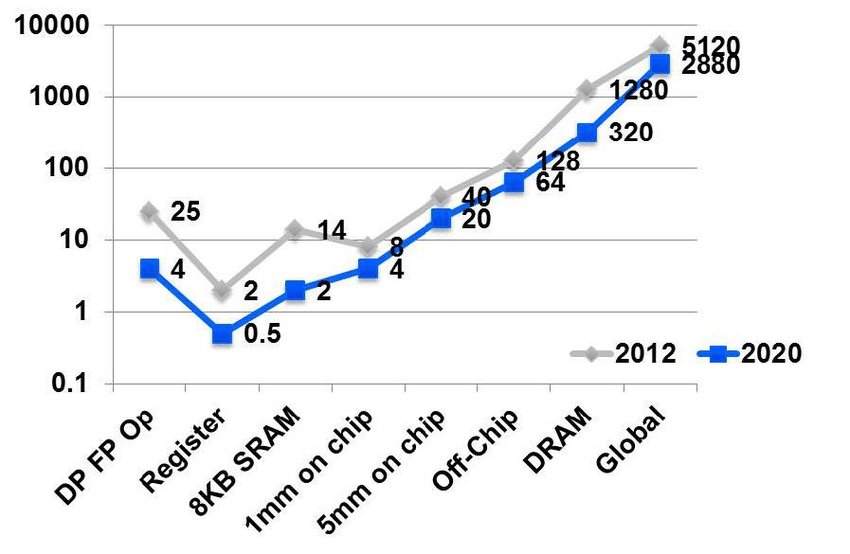
\includegraphics[width=10cm]{images/energy_pj.png}
            \caption{\label{fig:energy_pj} Coût énergétique, en picojoules (pJ) par opération à virgule flottante de 64 bits, pour diverses opérations courantes dans un ordinateur. La ligne supérieure (grise) représente le coût énergétique des opérations sur un processeur utilisé en 2012. La ligne inférieure (bleue) prévoit les coûts énergétiques en 2020 \cite{Leland2014}.}
            \end{figure}
            
                

        
        \paragraph{Le cas du supercalculateur Summit.} 
        
            Pour étudier la contrainte énergétique dans l'élaboration d'une plateforme Exascale, nous étudions certaines caractéristiques du supercalculateur Summit présentées dans le \autoref{tab:summit_analysis}. Ce dernier est classé numéro un au Top500 de novembre 2019 (voir \autoref{sec:Top500}). Il est aussi le premier supercalculateur du classement du Green500 consommant plus de 10 MW  (classé 5e en novembre 2019). Pour appréhender l'importance des efforts à fournir pour construire un supercalculateur capable d'exécuter $10^{18}$ opérations par seconde pour une application réelle, nous comparons l'efficacité énergétique de Summit avec celle d'un supercalculateur Exascale pour l'exécution du benchmark HPL.
        
            \begin{table}
            \centering
            \resizebox{\textwidth}{!}{%
            \begin{tabular}{|l|c|c|c|c|c|}
            \hline
            \rowcolor[HTML]{EFEFEF} 
            \textbf{Supercalculateur} & \textbf{\begin{tabular}[c]{@{}c@{}}Consommation\\ (MW)\end{tabular}} & \textbf{\begin{tabular}[c]{@{}c@{}}Perf. Linpack\\ (exaFLOPS)\end{tabular}} & \textbf{\begin{tabular}[c]{@{}c@{}}Efficacité énergétique\\ (GFLOP/watt)\end{tabular}} & \textbf{\begin{tabular}[c]{@{}c@{}}Budget énergétique\\ (pJ/opération)\end{tabular}} & \textbf{\begin{tabular}[c]{@{}c@{}}Conso. Linpack\\ (pJ/bit)\end{tabular}} \\ \hline
            \cellcolor[HTML]{EFEFEF}\textbf{Summit} & 10 & 0.200 & 20 & 50 & 0.25 \\ \hline
            \cellcolor[HTML]{EFEFEF}\textbf{Projet Exascale} & 20 - 30 & 1 & 50 - 33 & 20 - 30 & 0.1 - 0.15 \\ \hline
            \end{tabular}%
            }
            \caption{Comparaison de l'efficacité énergétique du supercalculateur Summit et de l'efficacité théorique d'une plateforme exascale\textbackslash{}cite\{Bergman2018\}.}
            \label{tab:summit_analysis}
            \end{table}
    
    
            Pour fonctionner, Summit a besoin d'une puissance de 10 MW. En novembre 2019, il a atteint une performance de 200 pétaFLOPS ($10^{15}$ \gls{FLOPS}) lors de l'exécution du benchmark Linpack. Son efficacité énergétique est donc de 20 GFLOP/watt. Un supercalculateur exaflopique consommant entre 20 et 30 MW aurait quant à lui, une efficacité énergétique comprise entre 33 et 50 GFLOP/watt. Le défi est donc de construire une plateforme 5 fois plus puissante tout en étant deux fois plus efficace énergétiquement. Cependant, le défaut du benchmark Linpack est qu'il ne reflète pas le comportement des applications industrielles. En effet, contrairement aux applications réelles, il ne nécessite aucune communication entre les noeuds, et les instructions sont réalisées sur des données présentes dans le cache. Atteindre un exaFLOPS sur le benchmark HPL sera bien plus facile que d'atteindre la même performance avec une application réelle dont la consommation est principalement due aux déplacements mémoires. Pour mieux appréhender l'impact énergétique des déplacements mémoires, nous calculons l'efficacité énergétique des deux supercalculateurs étudiés en joule/FLOP:
            \begin{equation}
                 \frac{FLOPS}{watt}  =  \frac{\frac{FLOP}{seconde}}  { \frac{joule}{second}} =  \frac{FLOP}{joule}
            \end{equation}
            Nous calculons ainsi le \textit{budget} disponible pour exécuter une opération flottante: 50 pJ pour Summit, contre 20 pJ et 30 pJ pour le supercalculateur Exascale. En moyenne, l'application exécute des instructions vectorielles de 200 bits \footnote{Source - \url{https://insidehpc.com/2019/07/flexibly-scalable-high-performance-architectures-with-embedded-photonics/}}. L'énergie dépensée par Summit pour calculer un bit est alors de 0.25 pJ. Pour une plateforme exascale, ce budget énergétique serait alors compris en 0.1 et 0.15 pJ/bit.
            
            Un accès à la mémoire se compte en centaine de picojoules par bit et en millier lorsqu'il s'agit de communication entre deux noeuds de calculs. Lorsque l'énergie disponible est de 0.1 pJ/bit et qu'un accès mémoire peut dépasser de cent fois ce budget, il est facile de comprendre que l'essentiel des innovations doivent se porter sur l'amélioration des communications (à l'intérieur des serveurs, mais aussi à l'extérieur) que ce soit par l'utilisation de nouvelles technologies ou d'une restructuration des microarchitectures. Les applications et les algorithmes doivent eux optimiser l'utilisation des données locales pour tirer profit des principes de localité (voir \autoref{sec:locality}).


    \subsubsection{La complexité}\label{sec:edl_chal_complexite}
    %%%%%%%%%%%%%%%%%%%%%%%%%%%%%%%%%%%%%%%%%%%%%%%%%%%%%%%%%%%%%%%%%%%%%%%%
    %%%%%%%%%%%%%%%%%%%%%%%%%%%%%%%%%%%%%%%%%%%%%%%%%%%%%%%%%%%%%%%%%%%%%%%%
        
        Comme présentées dans l'\aref{chap:sota:materiel}, les architectures des ordinateurs ont reçu de nombreuses améliorations au fil des ans. Ces améliorations se sont additionnées et ont permit le développement des processeurs tels que nous les connaissons aujourd'hui: une hiérarchie mémoire, plusieurs coeurs (logique et physique), un pipeline comportant souvent plus de dix étapes, des systèmes d'exécution dans le désordre ou encore de préchargement mémoire. 
        
        La complexification est aussi présente dans le logiciel. Pour tirer parti des fonctionnalités offertes par le matériel, plusieurs modèles de programmation sont utilisés pour par exemple exploiter la mémoire partagée et distribuée ou utiliser les différents coeurs d'un processeur. En fonction des tâches à réaliser, plusieurs langages peuvent être utilisés dans une même application (C, C++, fortran, python, cuda...). La programmation \textbf{efficace} d'un supercalculateur est ainsi devenue une tâche très difficile. La complexification du matériel et du logiciel a un fort impact sur la performance des applications qui parviennent rarement à exploiter une part significative de la performance disponible. La performance d’une même application peut fortement varier à cause d’une subtilité (la configuration du BIOS, un réglage du système d’exploitation). Certaines technologies (FPGA, GPU) ne sont pas envisagées par des entreprises, car l'adaptation de leurs applications pour fonctionner sur celles-ci est très difficile. Pour s'extraire de la complexité grandissante des plateformes HPC et de leur gestion, de plus en plus d'utilisateurs se tournent vers des solutions dématérialisées telles que le \textit{cloud}.
        
        %Dans le classement du Top500, on remarque ainsi que les supercalculateurs atteignent rarement plus de 80\% d'efficacité sur une application simple comme Linpack\cite{Dongarra2003}. Pour des applications réelles, cette efficacité est encore plus faible, parfois inférieure à 10\%\cite{Oliker2005}. 
        %La complexité des architectures a aussi un impact sur l'efficacité énergétique des plateformes, par exemple le mécanisme de prédiction de branchement ou l'agrandissement des différents niveaux du \textit{pipeline} (voir \autoref{sec:pipeline}).
        
        \paragraph{La sécurité.} La complexité du matériel et des couches logicielles représente un grand risque d'exploitation de faille de sécurité. Les applications utilisent de nombreuses librairies qui peuvent présenter des failles, et la difficulté de les mettre à jour (pour la stabilité des applications) peut permettre aux attaquants d'exploiter ces failles. L'accumulation de fonctionnalités a aussi rendu ces architectures sujettes à différentes attaques. En 2018, les chercheurs de Google \cite{kocher2018spectre} ont découvert une faille majeure dans le prédicteur de branchement des processeurs Intel (voir \autoref{sec:micro}). Aujourd'hui, les supercalculateurs sont rarement directement connectés au réseau internet, rendant difficile l'attaque de ces plateformes. Cependant, la vision exascale présentée dans le début du chapitre implique la collecte de données et le traitement des données au plus proche de la source de leur création ainsi que l'acheminement de certains résultats vers les centres de calculs, exposant de nombreux lieux d'attaque. Il n’est pas envisageable d'utiliser des voitures autonomes possédant des processeurs, des mémoires, des dizaines de couches logicielles pouvant être attaquées. De même, les données personnelles, telles que les données médicales enregistrées par les montres connectées sont très sensibles.
    
        
        \paragraph{Passage à l'échelle.} Pour obtenir un supercalculateur exascale, il est techniquement possible de construire 5 supercalculateurs de la puissance du Summit et d’agréger leur performance. Cependant, pour les raisons de coût, principalement lié à la consommation énergétique, cette solution n’est pas envisageable. À une telle échelle, le nombre de serveurs serait si important (supérieur à 30000) que des problèmes insoupçonnés à des tailles moindres feraient leur apparition. Les pannes des matériels, les congestions de réseaux et la capacité des applications à utiliser un grand nombre de serveurs impacteraient leur performance rendant le supercalculateur très inefficace. En effet, la programmation parallèle nécessite la synchronisation des ressources à différentes étapes du calcul pour partager des résultats intermédiaires. Ainsi, les pannes matérielles d'une seule ressource de calcul ont de forts impacts sur la performance des applications de calculs parallèles. 
        %Ces infrastructures seront utilisées pour exécuter des applications pendant plusieurs heures ou mêmes jours. Il est donc nécessaire de développer des systèmes de reprises suite à une erreur sans avoir à tout recommencer \cite{farjallah2014preparing} grâce à des mécanismes de point de contrôle (\textit{checkpoint}) \cite{Zheng2012}
        

    \subsubsection{Les nouvelles technologies}\label{sec:edl_chal_new_techno}
    %%%%%%%%%%%%%%%%%%%%%%%%%%%%%%%%%%%%%%%%%%%%%%%%%%%%%%%%%%%%%%%%%%%%%%%%    %%%%%%%%%%%%%%%%%%%%%%%%%%%%%%%%%%%%%%%%%%%%%%%%%%%%%%%%%%%%%%%%%%%%%%%%

        Nous avons montré précédemment que les utilisateurs étaient en demande de puissance de calcul supplémentaire. 
        Le classement du Top500,  réalisé tous les 6 mois, permet de classer les plateformes les plus récentes. Les nombreux supercalculateurs construits chaque année rentrent au classement, remplaçant les anciennes plateformes moins performantes. Sur la \autoref{fig:edl_top500_age}, nous constatons que l'âge moyen du Top500 a doublé en quelques années indiquant la difficulté à produire des supercalculateurs plus performants. Alors que l'âge moyen du classement oscillait autour de 7 mois pour les 23 premières années du classement, il a dépassé les 15 mois depuis les années 2013. Ces deux constats montrent que les utilisateurs de HPC ne renouvellent plus leurs supercalculateurs, car ils ne trouvent plus de solutions matérielles suffisamment intéressantes pour motiver de nouveaux investissements. De nouvelles technologies doivent émerger pour obtenir de réels gains de performance. L'histoire récente nous a prouvé que ce chemin était le bon avec l'utilisation des GPU (ou d'accélérateurs dédiés comme les TPU de Google) pour accélérer les applications d'apprentissage par machine. Les pressions économiques et énergétiques présentées précédemment nous indiquent que de nombreuses avancées doivent être réalisées dans tous les domaines touchant au HPC: les processeurs, les accélérateurs, les mémoires, les réseaux ou bien la partie logiciel. 
        
        
                  
            \begin{figure}
                \center
                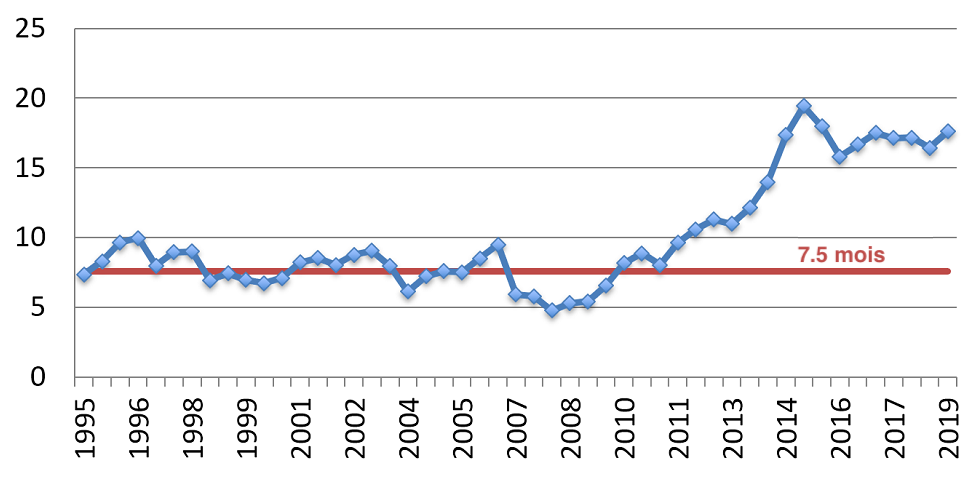
\includegraphics[width=10cm]{images/edl_top500_age.png}
                \caption{\label{fig:edl_top500_age} Âge moyen des supercalculateurs classés au Top500 \cite{Strohmaier2018}.}
            \end{figure}
       
        %Exemple de nouveauté
        

        \paragraph[Explosion cambrienne] {Explosion ``cambrienne'' \footnote{L’explosion cambrienne désigne l'apparition soudaine (à l'échelle des temps géologiques) de la plupart des grands embranchements actuels des animaux pluricellulaires ainsi qu'une grande diversification des espèces animales, végétales et bactériennes (wikipédia).}}
        
            De nouvelles technologies existent ou sont en cours de développement. Dans la \autoref{sec:oppo_new_tech}, nous montrons que de nombreuses solutions matérielles, technologiques et logicielles peuvent être utilisées. Des accélérateurs et des mémoires très spécifiques pourront être utilisés. Les utilisateurs de HPC et les architectes doivent alors connaître les besoins de leurs applications pour choisir quelles technologies utiliser (type et quantité de mémoire, utilisation d'accélérateurs). Si ces nouvelles technologies peuvent être une réelle opportunité pour l'élaboration de plateformes plus puissantes et plus efficaces, elles sont aussi un défi. En effet, jusqu’à récemment, la majorité des plateformes étaient construites de façon similaire: un processeur x86 pouvant être associé à un GPU (voir \autoref{sec:edl_hpc_hetero}). Si les applications obtenaient de faibles performances, il était difficile de s'orienter vers d'autres solutions alors inexistantes. La majorité des supercalculateurs sont utilisés par différents utilisateurs et exécutent différents types d'applications. Le choix des technologies utilisées doit alors prendre en compte ces différentes applications pour construire la plateforme la plus efficace possible. Souvent ces centres de calculs seront hétérogènes avec différents processeurs.
        
        \paragraph{Nouveautés au Top500.} En étudiant le classement du Top500, nous constatons les premiers signes de l'évolution des plateformes qui utilisent de nouveaux types de processeurs ou d'accélérateurs (voir \autoref{fig:new_proc}). En novembre 2019, trois supercalculateurs classés à la 84e, 72e et 116e place étaient équipés de processeur Sparc64 XIfx \cite{Yoshida2018}. Ce processeur est produit par Fujitsu et possède 34 coeurs (dont deux réservés en priorité au système d'exploitation et à la gestion des communications). Il possède 24 Mb de cache L2 et atteint une performance de 1,1 téraFLOPS (voir \autoref{fig:edl_sparc64}). Pour atteindre de hautes performances sur des applications réelles, le processeur est doté d'une mémoire empilée HMC de 32 GB \cite{Garg2017}. Concernant les accélérateurs, nous pouvons citer le coprocesseur Matrix-2000 qui a permis de doubler la puissance du supercalculateur chinois Tianhe-2 en remplaçant les anciens accélérateurs KNL par une nouvelle architecture développée exclusivement pour lui. Cet accélérateur 64 bits produit par NUDT, possède 128 coeurs RISC à 1,2 GHz permettant d'atteindre une performance crête de 4,92 téraFLOPS pour une enveloppe thermique de 240W. Quatre groupes de 32 coeurs sont reliés à la mémoire avec un total de 8 canaux mémoire (voir \autoref{fig:edlp_matrix_2000}). 
        
          
        \begin{figure}[t!]
            \centering
            \begin{subfigure}[t]{0.48\textwidth}
                \centering
                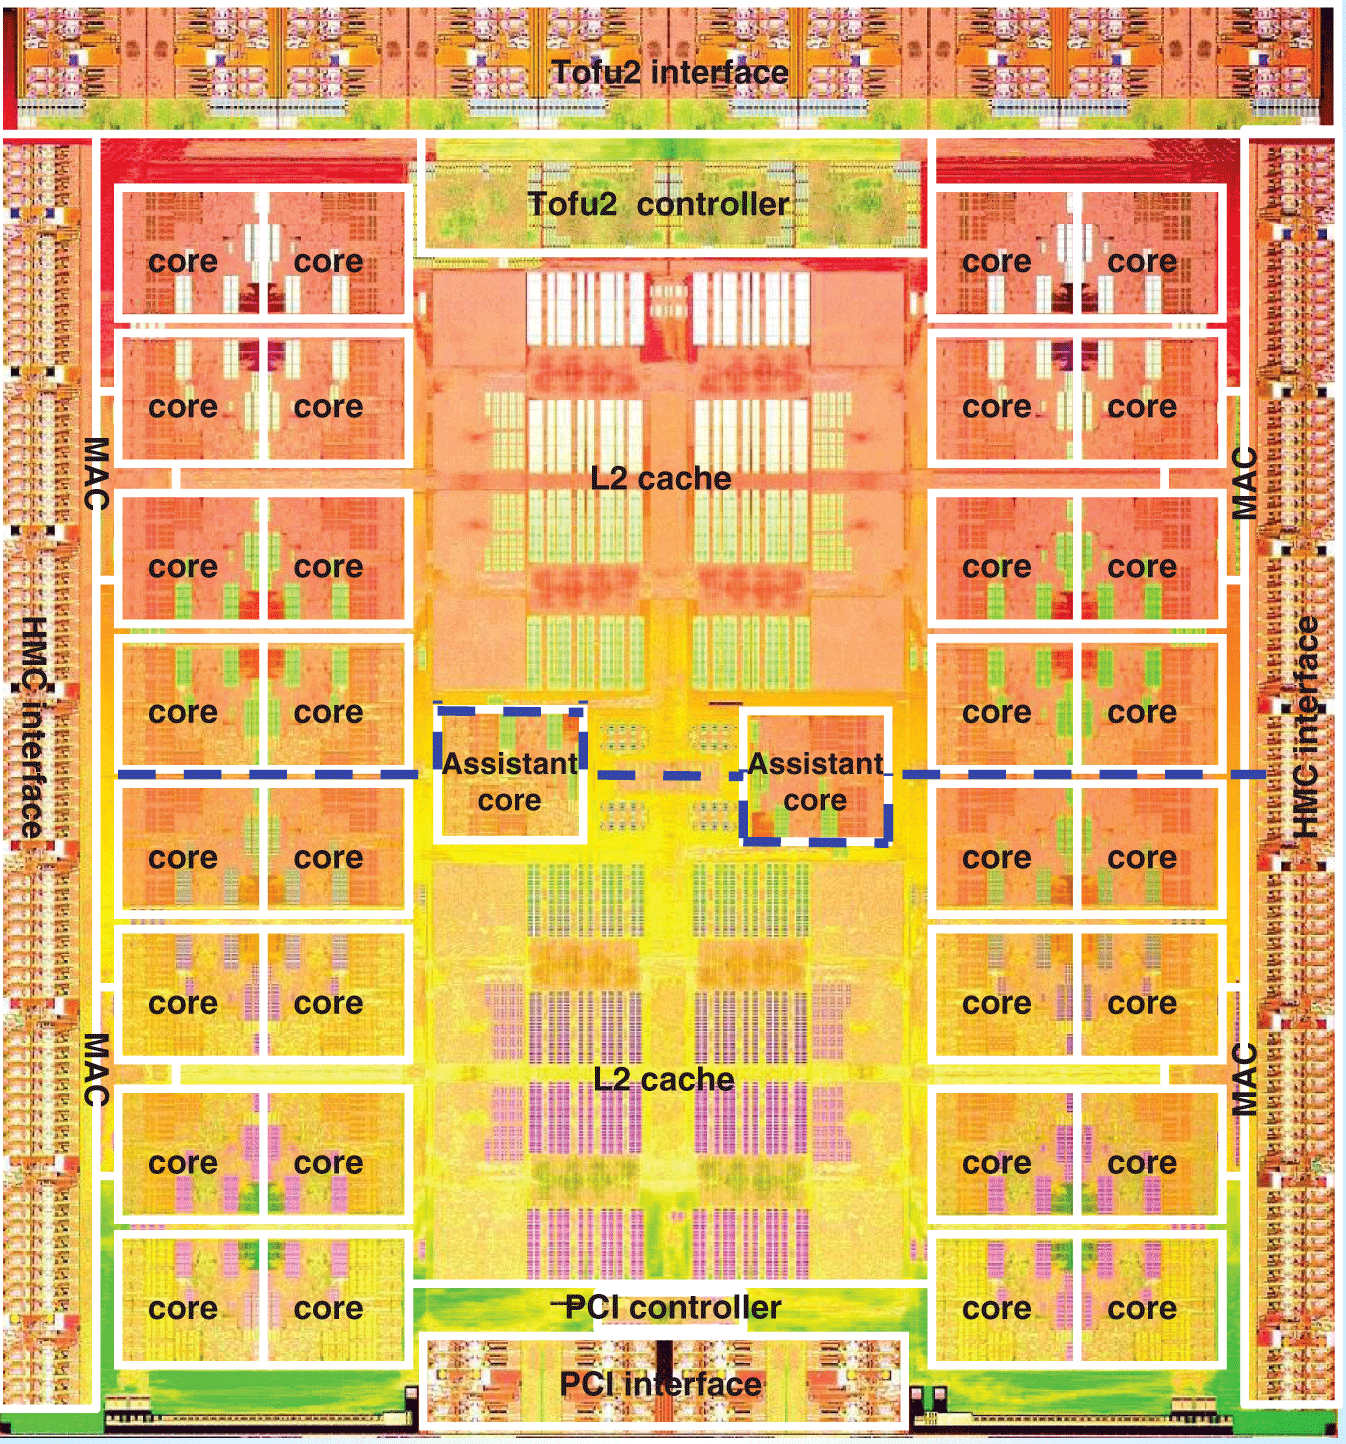
\includegraphics[width=0.9\linewidth]{images/edl_sparc64.png}
                \caption{\label{fig:edl_sparc64} Le processeur Sparc64 est produit par Fujitsu et utilise une mémoire empilée HMC\cite{7021857}.}
            \end{subfigure}\hfill
            \begin{subfigure}[t]{0.48\textwidth}
                \centering
                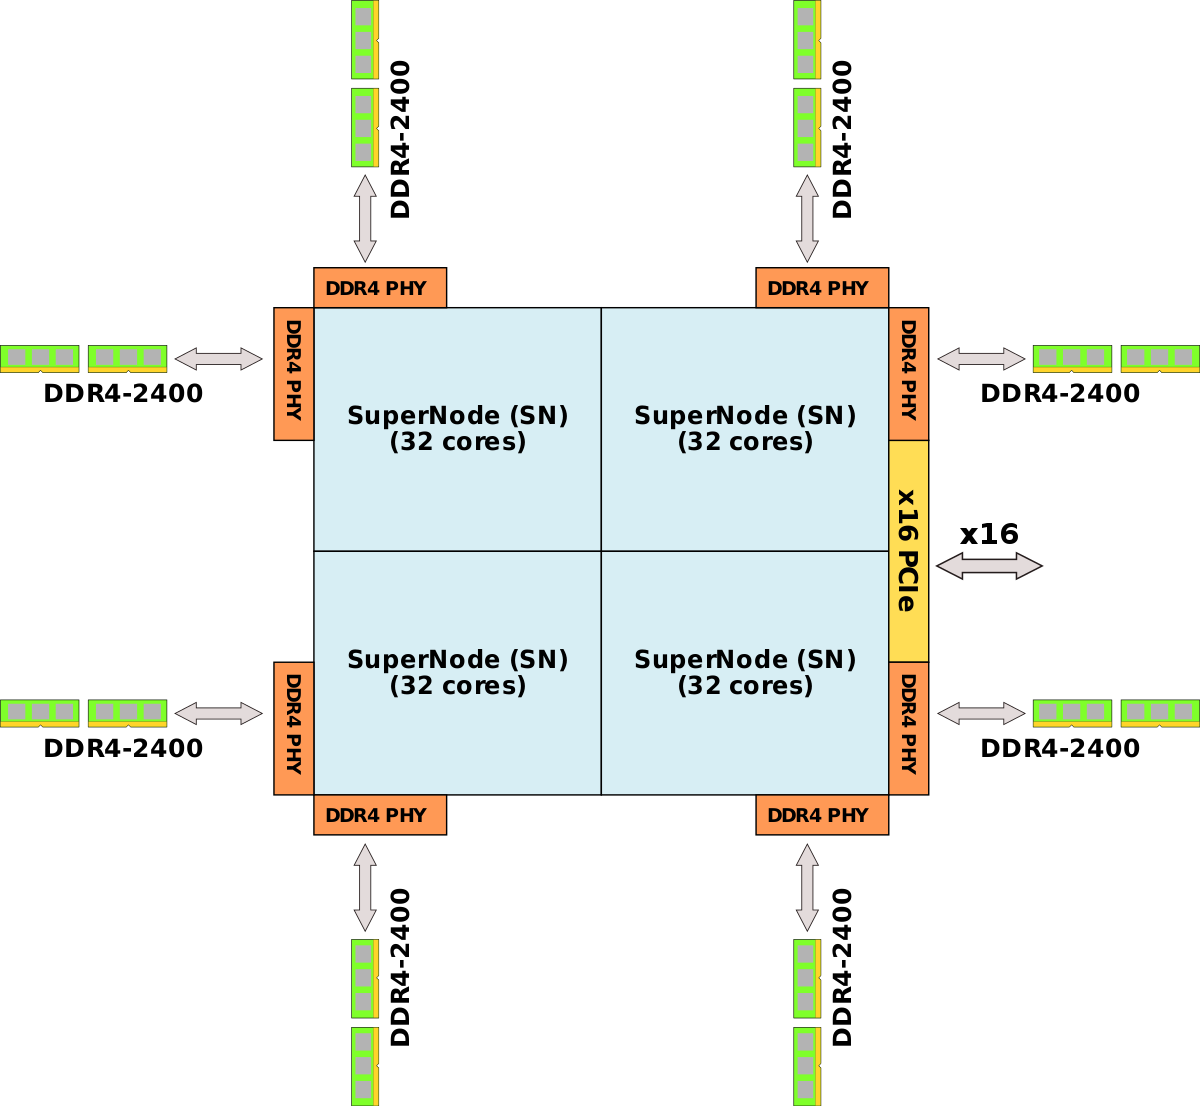
\includegraphics[width=\linewidth]{images/edlp_matrix_2000.png}
                \caption{\label{fig:edlp_matrix_2000}Le coprocesseur Matrix 2000 possède 128 coeurs et 8 canaux mémoires.}
            \end{subfigure}
            \caption{\label{fig:new_proc} De nouvelles architectures sont utilisées dans les supercalculateurs classés au Top500.}
        \end{figure}

           
    \subsubsection{Rapidité de l'évaluation des nouvelles technologies} \label{sec:edl_chal_vitesse}
    %%%%%%%%%%%%%%%%%%%%%%%%%%%%%%%%%%%%%%%%%%%%%%%%%%%%%%%%%%%%%%%%%%%%%%%%    %%%%%%%%%%%%%%%%%%%%%%%%%%%%%%%%%%%%%%%%%%%%%%%%%%%%%%%%%%%%%%%%%%%%%%%%
        
        Face à l'arrivée de ces nombreuses technologies, les entreprises doivent rapidement être capables d'évaluer leurs qualités et leurs défauts et quantifier leur adéquation avec leurs applications. Les évolutions récentes sont très rapides avec le développement de dizaines de modèles de mémoire, de nouveaux accélérateurs et de processeurs. Certaines technologies encore en développement sont déjà dépassées par l’annonce de nouvelles technologies.
        
        Une technologie émergente, très performante pour une application, avec des consommations énergétiques ou un coût très faible peut permettre à une industrie de faire un bond de performance dans un domaine. Grâce à ces technologies, l'économie d'un domaine peut être fortement modifiée en permettant de réaliser des simulations dix fois plus rapidement ou en divisant leur coût du même facteur.
                
        La vitesse de décision et d'utilisation d'une nouvelle technologie dans notre société mondialisée est cruciale. Les entreprises doivent donc disposer de moyens (techniques et financiers) pour se tenir à l'état de l'art des technologies. Le développement de partenariat (avec des universités par exemple) est une des clefs permettant de s’assurer de la capacité des entreprises à ingérer ces nouvelles technologies.


    \subsubsection{L'expertise}\label{sec:edl_chal_expertise}
    %%%%%%%%%%%%%%%%%%%%%%%%%%%%%%%%%%%%%%%%%%%%%%%%%%%%%%%%%%%%%%%%%%%%%%%
    %%%%%%%%%%%%%%%%%%%%%%%%%%%%%%%%%%%%%%%%%%%%%%%%%%%%%%%%%%%%%%%%%%%%%%%%

        Pour construire les plateformes de demain, il est nécessaire de pouvoir qualifier les nouvelles architectures émergentes. Cette qualification devant se faire rapidement sur des dizaines d'architectures différentes, il est important pour les acteurs du HPC d'avoir les moyens adéquats pour mener à bien cette mission. Pour motiver les choix à entreprendre, une modélisation économique des performances ($FLOP/\$$, $GB/s/\$$) doit pouvoir être réalisée. Une fois les architectures sélectionnées, les programmeurs doivent être capables d'extraire une part importante des performances disponibles. Les architectures ciblées pouvant être très différentes des processeurs x86 largement utilisés aujourd'hui, les programmeurs doivent avoir de solides connaissances et les outils adaptés, sans quoi certaines architectures devront être abandonnées. Les outils à leur disposition doivent leur permettre d'établir un profil des besoins de son application pour pouvoir caractériser et sélectionner les différentes plateformes. Pour étudier son application et valider leur performance une fois le code porté, il est nécessaire d'avoir des outils facilement utilisables sur différentes plateformes (et différentes microarchitectures).
        
        Les FPGA (Field Programmable Gate Array) en sont un bon exemple. Cette technologie permet de faire des périphériques très performants et très efficaces en termes de consommation électrique. L'idée principale étant de laisser au programmeur le développement complet du circuit électronique pour qu'il corresponde parfaitement à son besoin. Mais la programmation de tels circuits est très complexe et demande des mois, souvent des années pour des codes industriels, pour être réalisée. Ainsi, malgré l'efficacité, prouvée, de cette technologie, les entreprises ne s'y lancent pas à cause des coûts engendrés par l'achat du matériel et la taille des équipes requises pour programmer et supporter les applications. 
        
        
        %\paragraph{Programmation des supercalculateurs.} Dans la \autoref{sec:edl_chal_complexite} nous avons rappelé la complexité de programmer un supercalculateur, qui nécessite l'utilisation de plusieurs modèles de programmation et souvent de plusieurs langages. L'apparition de plateforme hétérogène (voir \autoref{sec:edl_hpc_hetero}) va rendre la tâche d'autant plus difficile. Pour l'aider, le programmeur doit avoir à sa disposition une couche logicielle et un modèle de programmation pour l’aider, lui permettant de se concentrer seulement sur le développement de son algorithme. Les outils de répartition de charges doivent être améliorés pour prendre en compte l'hétérogénéité des architectures disponible.
        
        
        \paragraph{Optimisation des codes.} 
            
            Le défi de l’exascale ne vient pas seulement du matériel et des technologies que nous allons utiliser comme le soulignent certains travaux \cite{barrett2012navigating}. Il  nécessite aussi de repenser une grande partie des logiciels. Cette partie est très délicate, car les applications atteignent souvent plusieurs dizaines de milliers de lignes de codes. Changer un compilateur ou un debugger peut alors s’avérer plus complexe qu'il n’y paraît. Pour atteindre les meilleures performances possibles, les programmeurs doivent être capables d'écrire des applications optimisées pour les architectures utilisées. Pour cela, il est nécessaire de restructurer le code ou d'utiliser d'autres algorithmes pour tirer parti des caractéristiques du matériel (hiérarchie de cache, taille de la mémoire, nombre de coeurs...). Des optimisations telles que le découpage en bloc \cite{Xue2012} ou le \textit{time squewing} \cite{Wonnacott2002} existent et ont prouvé leur efficacité. Cependant, leur implémentation sur des applications industrielles peut être très fastidieuse et les performances atteintes peuvent être différentes de celles attendues. 
            
            %Cette partie pourrait être laissée au compilateur, mais il est très difficile de proposer un tel compilateur générique étant capable de les implémenter. Les compilateurs ont un rôle central dans le développement et l’exécution des applications, car ils sont l’intermédiaire entre le programmeur et le matériel. Leur efficacité à générer du code de qualité est primordiale pour tirer le maximum de performances de ces architectures complexes.

        %Algo
        \paragraph{Adapter les algorithmes.} Une source (presque) inépuisable d'accélération des applications vient de l'utilisation de nouveaux algorithmes. La \autoref{fig:edl_new_algo}, montre comment l'utilisation de nouvelles méthodes mathématiques permet d'accélérer de plusieurs facteurs la résolution d'une équation de poisson. Une application nécessitant 6 mois de calculs en 1947 peut être résolue grâce à une méthode multigrille \cite{Brandt1982} en moins d'une seconde.
            
            Pour réduire le nombre d’opérations lors de la multiplication de matrices pour les algorithmes d’apprentissage par machine, plusieurs techniques peuvent être utilisées \cite{Sze2017}: la transformée de Fourier rapide \cite{Vasilache2014}, l’algorithme de Strassen \cite{Cong2014} ou encore l'algorithme de Coppersmith-Winograd \cite{Li2016}. En fonction des caractéristiques de l’architecture (stockage disponible), du besoin de stabilité numérique, ou de la taille des matrices utilisées, chaque méthode a ses avantages et inconvénients. Le compilateur peut alors choisir la meilleure technique à utiliser en fonction de ces paramètres.
    
            \begin{figure}
            \center
            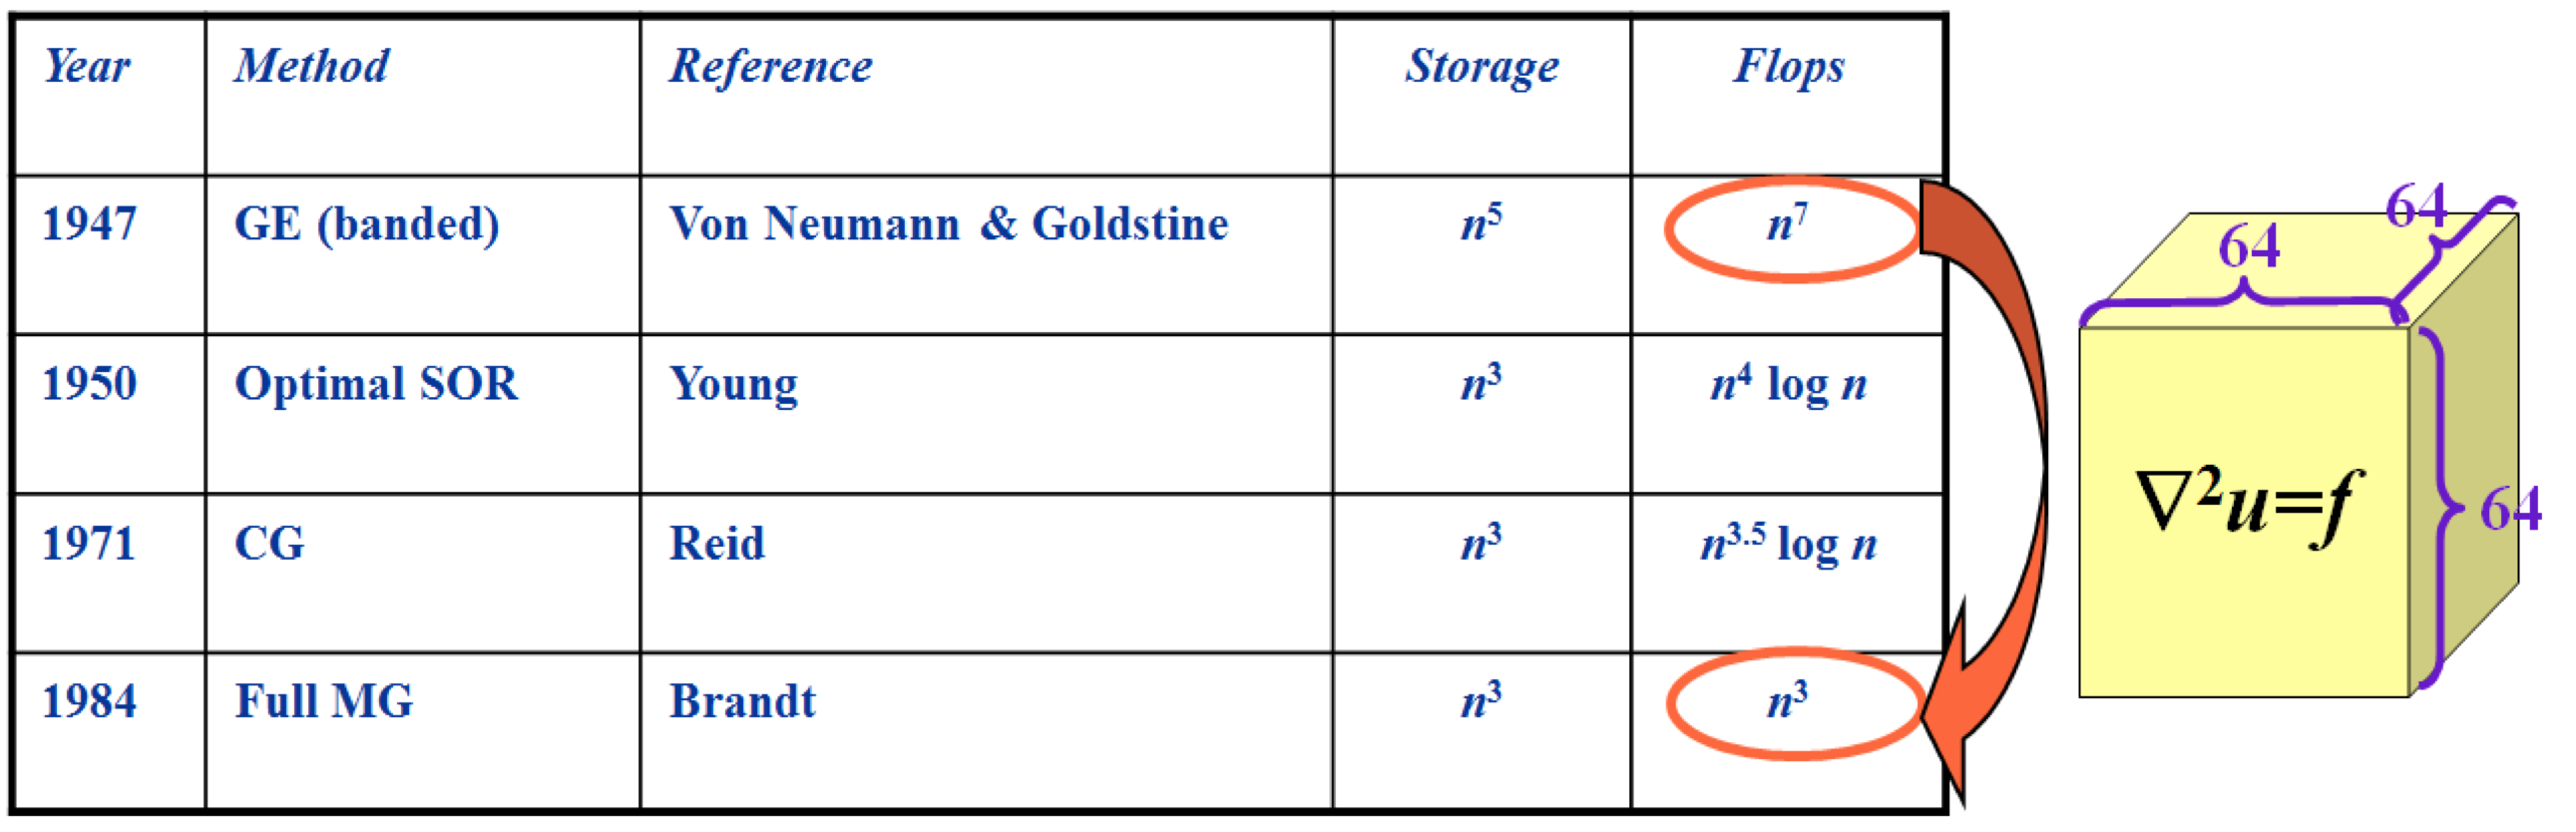
\includegraphics[width=14cm]{images/edl_new_algo.png}
            \caption{\label{fig:edl_new_algo} L'utilisation de nouvelle méthodes mathématiques a permis de réduire de plusieurs facteurs la quantité de stockage (\textit{storage}) et le nombre de calculs nécessaires (\textit{flops}) pour la résolution d'une équation de poisson\protect\footnotemark.}
            \end{figure}
            \footnotetext{Tableau extrait de la présentation de David Keyes - \url{http://www.cs.odu.edu/~keyes/talks/SC_IMI.ppt}}

            Pour les plateformes exascale, les algorithmes doivent être adaptés à certaines contraintes. Le coût des déplacements des données, en énergie et en temps, doit être le moteur de leur développement et de leurs améliorations. En effet, le coût énergétique de l'exécution d’une opération flottante peut être considéré comme gratuit quand on le compare au coût du déplacement des données. La plus grande pénalité venant des communications entre les noeuds de calculs, les algorithmes doivent réduire au maximum ces communications en découpant stratégiquement le jeu de données. Il peut même être avantageux de recalculer certains résultats localement, plutôt que de les communiquer entre deux serveurs. L'algorithme de Strassen \cite{Lipshitz2012} permet par exemple la multiplication de deux matrices sans échanges de données. Ces techniques ont un gain double: elles sont plus rapides, car l’exécution n’est pas pénalisée par la performance du réseau, et elles sont plus efficaces énergétiquement, car elles ne payent pas le coût de la communication des données. Cependant, ces méthodes peuvent entraîner des problèmes de stabilité numérique \cite{khabou2013dense}. 
                        

        \paragraph{Challenge.}  
        
            La complexification des applications et du matériel ajoutée au manque de connaissances et d'outils des utilisateurs se traduit par une mauvaise utilisation des plateformes évoquée dans la \autoref{sec:Top500}. Bien que la recherche ait réalisé de nombreuses découvertes, peu d'entre elles sont réellement appliquées sur les codes industriels. La loi de Moore assurant une évolution constante des performances des architectures, l’analyse et l’optimisation des codes ont été laissées de côté. Les investissements réalisés dans le développement des matériels se sont faits au détriment des logiciels. Aujourd'hui, nous constatons un manque de connaissances fines des architectures dû à leur complexité croissante ainsi que le manque d'outils adéquats pour réaliser les optimisations nécessaires.
        
